%%%%%%%%%%%%%%%%%%%%%%%%%%%%%%%%%%%%%%%%%
% The Legrand Orange Book
% LaTeX Template
% Version 3.1 (February 18, 2022)
%
% This template originates from:
% https://www.LaTeXTemplates.com
%
% Authors:
% Vel (vel@latextemplates.com)
% Mathias Legrand (legrand.mathias@gmail.com)
%
% License:
% CC BY-NC-SA 4.0 (https://creativecommons.org/licenses/by-nc-sa/4.0/)
%
% Compiling this template:
% This template uses biber for its bibliography and makeindex for its index.
% When you first open the template, compile it from the command line with the 
% commands below to make sure your LaTeX distribution is configured correctly:
%
% 1) pdflatex main
% 2) makeindex main.idx -s indexstyle.ist
% 3) biber main
% 4) pdflatex main x 2
%
% After this, when you wish to update the bibliography/index use the appropriate
% command above and make sure to compile with pdflatex several times 
% afterwards to propagate your changes to the document.
%
%%%%%%%%%%%%%%%%%%%%%%%%%%%%%%%%%%%%%%%%%

%----------------------------------------------------------------------------------------
%	PACKAGES AND OTHER DOCUMENT CONFIGURATIONS
%----------------------------------------------------------------------------------------

\documentclass[
	11pt, % Default font size, select one of 10pt, 11pt or 12pt
	fleqn, % Left align equations
	a4paper, % Paper size, use either 'a4paper' for A4 size or 'letterpaper' for US letter size
	%oneside, % Uncomment for oneside mode, this doesn't start new chapters and parts on odd pages (adding an empty page if required), this mode is more suitable if the book is to be read on a screen instead of printed
]{LegrandOrangeBook}
% Book information for PDF metadata, remove/comment this block if not required 
\hypersetup{
	pdftitle={Title}, % Title field
	pdfauthor={Author}, % Author field
	pdfsubject={Subject}, % Subject field
	pdfkeywords={Keyword1, Keyword2, ...}, % Keywords
	pdfcreator={LaTeX}, % Content creator field
}

\addbibresource{sample.bib} % Bibliography file

\definecolor{ocre}{RGB}{243, 102, 25} % Define the color used for highlighting throughout the book

\chapterimage{orange1.jpg} % Chapter heading image
\chapterspaceabove{6.5cm} % Default whitespace from the top of the page to the chapter title on chapter pages
\chapterspacebelow{6.75cm} % Default amount of vertical whitespace from the top margin to the start of the text on chapter pages

%----------------------------------------------------------------------------------------

\pgfplotsset{compat=1.18}

\begin{document}

%----------------------------------------------------------------------------------------
%	TITLE PAGE
%----------------------------------------------------------------------------------------

\titlepage % Output the title page
	{
\includegraphics[width=\paperwidth]{background.pdf}} % Code to output the background image, which should be the same dimensions as the paper to fill the page entirely; leave empty for no background image
	{ % Title(s) and author(s)
		\centering\sffamily % Font styling
		{\Huge\bfseries Nonlinear Control Theory\par} % Book title
		\vspace{16pt} % Vertical whitespace
		{\LARGE A Condensed Guide\par} % Subtitle
		\vspace{24pt} % Vertical whitespace
		{\huge\bfseries Rakshan\par} % Author name
	}

%----------------------------------------------------------------------------------------
%	COPYRIGHT PAGE
%----------------------------------------------------------------------------------------

\thispagestyle{empty} % Suppress headers and footers on this page

~\vfill % Push the text down to the bottom of the page

\noindent Copyright \copyright\ 2025 Rakshan\\ % Copyright notice

%\noindent \textsc{Published by Publisher}\\ % Publisher

%\noindent \textsc{\href{https://www.latextemplates.com/template/legrand-orange-book}{book-website.com}}\\ % URL

\noindent {\small
Licensed under the MIT License (the ``License''). You may not use this file except in compliance with the License.  

\medskip

Permission is hereby granted, free of charge, to any person obtaining a copy of this material and associated documentation files (the ``Material''), to deal in the Material without restriction, including without limitation the rights to use, copy, modify, merge, publish, distribute, sublicense, and/or sell copies of the Material, and to permit persons to whom the Material is furnished to do so, subject to the following conditions:

\medskip

The above copyright notice and this permission notice shall be included in all copies or substantial portions of the Material.

\medskip

\textsc{The Material is provided ``as is'', without warranty of any kind, express or implied}, including but not limited to the warranties of merchantability, fitness for a particular purpose and noninfringement. In no event shall the authors or copyright holders be liable for any claim, damages or other liability, whether in an action of contract, tort or otherwise, arising from, out of or in connection with the Material or the use or other dealings in the Material.
}\\


\noindent \textit{First Edition , August 2025} % Printing/edition date

%----------------------------------------------------------------------------------------
%	TABLE OF CONTENTS
%----------------------------------------------------------------------------------------

\pagestyle{empty} % Disable headers and footers for the following pages

\tableofcontents % Output the table of contents

\listoffigures % Output the list of figures, comment or remove this command if not required

\listoftables % Output the list of tables, comment or remove this command if not required

\pagestyle{fancy} % Enable default headers and footers again

\cleardoublepage % Start the following content on a new page

\part{PRELIMINARIES}
\chapterimage{orange2.jpg} % Chapter heading image
\chapterspaceabove{6.75cm} % Whitespace from the top of the page to the chapter title on chapter pages
\chapterspacebelow{7.25cm} % Amount of vertical whitespace from the top margin to the start of the text on chapter pages

\chapter{Introduction}\index{Introduction}

\section{Overview}\index{Overview}
This chapter introduces the basis for nonlinear control theory. We begin with linear time-invariant (LTI) systems, then define nonlinear systems and discuss equilibrium points. Phase plane analysis is carried out for both linear and nonlinear cases, followed by an extension to higher-order systems. Finally, illustrative examples are presented for better understanding.

\section{Linear Time-invariant Systems}\index{Linear Time-invariant Systems}
\begin{definition}[LTI System]
A linear time-invariant (LTI) system can be represented in state-space form as:
\begin{align}
    \dot{x}(t) &= A x(t) + B u(t), \\
    y(t) &= C x(t) + D u(t),
\end{align}
where $x(t)$ is the state vector, $u(t)$ the input, and $y(t)$ the output.
\end{definition}

\begin{example}[Spring–Mass–Damper System]

\begin{figure}[h!]
    \centering
    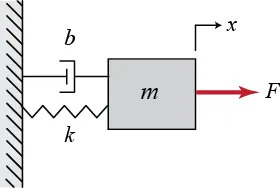
\includegraphics[width=0.35\textwidth]{Images/nonlinear/introduction/mass_spring_damper.jpg}
    \caption{Spring–mass–damper system with external force $F(t)$.}
    \label{fig:spring}
\end{figure}

Consider a mass $m$ attached to a spring (constant $k$) and damper (coefficient $b$), subject to an external force $F(t)$ as shown in the figure \ref{fig:spring}.  
The equation of motion is:
\begin{equation}
    m\ddot{x}(t) + b\dot{x}(t) + kx(t) = F(t).
\end{equation}

Defining the state vector as $x_1 = x(t)$ and $x_2 = \dot{x}(t)$, the system becomes:
\begin{align}
    \dot{x}_1 &= x_2, \\
    \dot{x}_2 &= -\tfrac{k}{m}x_1 - \tfrac{b}{m}x_2 + \tfrac{1}{m}F(t).
\end{align}

In matrix form:
\begin{equation}
\dot{x}(t) =
\begin{bmatrix}
0 & 1 \\
-\tfrac{k}{m} & -\tfrac{b}{m}
\end{bmatrix} x(t) +
\begin{bmatrix}
0 \\ \tfrac{1}{m}
\end{bmatrix} F(t),
\qquad
y(t) =
\begin{bmatrix}
1 & 0
\end{bmatrix} x(t).
\end{equation}
\end{example}

\section{Nonlinear Systems}\index{Nonlinear Systems}
\begin{definition}[Nonlinear System]
A general nonlinear system in state-space form is written as:
\begin{align}
    \dot{x} &= f\big(x,u,t\big), \\
    y &= g\big(x,u,t\big)
\end{align}
where $f(\cdot)$ and $g(\cdot)$ may depend explicitly on time $t$ in addition to the states $x$ and inputs $u$.
\end{definition}

\begin{example}[Spring–Mass–Damper with Nonlinear Spring]
Consider again the spring mass damper system as shown in figure \ref{fig:spring}, but now the spring has a nonlinear restoring force:
\begin{equation}
    F_{\text{spring}}(x) = k_1 x + k_3 x^3,
\end{equation}
so that the equation of motion becomes:
\begin{equation}
    m\ddot{x}(t) + b\dot{x}(t) + k_1 x(t) + k_3 x^3(t) = F(t).
\end{equation}

Defining $x_1 = x(t)$ and $x_2 = \dot{x}(t)$, the state equations are:
\begin{align}
    \dot{x}_1(t) &= x_2(t), \\
    \dot{x}_2(t) &= -\tfrac{b}{m}x_2(t) - \tfrac{k_1}{m}x_1(t) - \tfrac{k_3}{m}x_1^3(t) + \tfrac{1}{m}F(t).
\end{align}

Compactly,
\begin{equation}
\dot{x}(t) =
\begin{bmatrix}
x_2(t) \\
-\tfrac{b}{m}x_2(t) - \tfrac{k_1}{m}x_1(t) - \tfrac{k_3}{m}x_1^3(t) + \tfrac{1}{m}F(t)
\end{bmatrix},
\qquad
y(t) = x_1(t).
\end{equation}
\end{example}

\subsection{Special Cases}\index{Nonlinear Systems!Special Cases}
\begin{itemize}
    \item \textbf{Unforced System ($u(t)=0$):}  
    When $F(t)=0$, the dynamics reduce to:
    \begin{equation}
        \dot{x}_1 = x_2, \qquad 
        \dot{x}_2 = -\tfrac{b}{m}x_2 - \tfrac{k_1}{m}x_1 - \tfrac{k_3}{m}x_1^3.
    \end{equation}

    \item \textbf{Autonomous System ($\dot{x}=f(x)$):}  
    If the system has no input and no explicit time dependence,
    \begin{equation}
        \dot{x}(t) = f\big(x(t)\big).
    \end{equation}
    For this example,
    \begin{equation}
        \dot{x} =
        \begin{bmatrix}
        x_2 \\
        -\tfrac{b}{m}x_2 - \tfrac{k_1}{m}x_1 - \tfrac{k_3}{m}x_1^3
        \end{bmatrix}.
    \end{equation}
\end{itemize}

\section{Equilibrium Points}\index{Equilibrium Points}

\begin{definition}[Equilibrium Point]
An equilibrium point of a dynamical system
\begin{equation}
    \dot{x} = f(x,u,t),
\end{equation}
is a point $x_e$ (with corresponding input $u_e$) such that the state does not change in time:
\begin{equation}
    f(x_e,u_e,t) = 0, \qquad \forall t.
\end{equation}
In other words, if the system starts at $(x_e,u_e)$, it remains there for all time when there is no disturbance.
\end{definition}

\begin{example}[Spring–Mass–Damper with Nonlinear Spring]
For the nonlinear spring–mass–damper system
\begin{equation}
    \dot{x}_1 = x_2, \qquad 
    \dot{x}_2 = -\tfrac{b}{m}x_2 - \tfrac{k_1}{m}x_1 - \tfrac{k_3}{m}x_1^3 + \tfrac{1}{m}F(t),
\end{equation}
the equilibrium points are obtained by solving
\begin{align}
    0 &= x_2, \\
    0 &= -\tfrac{b}{m}x_2 - \tfrac{k_1}{m}x_1 - \tfrac{k_3}{m}x_1^3 + \tfrac{1}{m}F.
\end{align}

Thus, the equilibria satisfy
\begin{equation}
    -k_1 x_1 - k_3 x_1^3 + F = 0, \qquad x_2 = 0.
\end{equation}

\end{example}

\section{First-order Autonomous Nonlinear Systems}\index{First-order Autonomous Nonlinear Systems}

We consider systems of the form
\begin{equation}
    \dot{x} = f(x).
\end{equation}

\subsection{Linear Case}\index{First-order Autonomous Nonlinear Systems!Linear Case}
For a linear system
\begin{equation}
    \dot{x} = a x,
\end{equation}
the solution is
\begin{equation}
    x(t) = e^{at} x(0).
\end{equation}

\begin{itemize}
    \item If $a < 0$, the solution decays to zero (stable equilibrium).
    \item If $a > 0$, the solution diverges from zero (unstable equilibrium).
\end{itemize}

\subsection{General Nonlinear Case}\index{First-order Autonomous Nonlinear Systems!General Nonlinear Case}
For a general nonlinear function $f(x)$, an explicit analytical solution is often not possible.  
Instead, we examine the qualitative behavior by plotting $\dot{x} = f(x)$ as a function of $x$.  

\begin{example}[Nonlinear Example]
Consider
\begin{equation}
    \dot{x} = \cos x.
\end{equation}
Equilibrium points are given by $\cos x = 0$, i.e.
\[
x = \tfrac{\pi}{2} + n\pi, \quad n \in \mathbb{Z}.
\]
\end{example}

\begin{center}
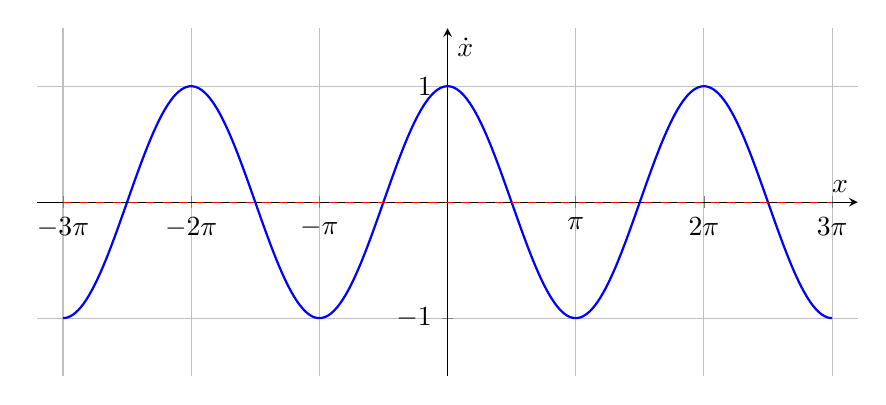
\begin{tikzpicture}[scale=1.0]
\begin{axis}[
    axis lines=middle,
    xlabel={$x$},
    ylabel={$\dot{x}$},
    domain=-3*pi:3*pi,
    samples=300,
    width=12cm,
    height=6cm,
    grid=both,
    xmin=-3.2*pi, xmax=3.2*pi,
    ymin=-1.5, ymax=1.5,
    xtick={-9.425,-6.283,-3.142,0,3.142,6.283,9.425},
    xticklabels={$-3\pi$,$-2\pi$,$-\pi$,0,$\pi$,$2\pi$,$3\pi$},
    ytick={-1,0,1}
]
\addplot[blue, thick] {cos(deg(x))};
\draw[dashed, red] (-3*pi,0) -- (3*pi,0); % equilibrium reference line
\end{axis}
\end{tikzpicture}
\end{center}

From the plot we observe:
\begin{itemize}
    \item Where $\dot{x} > 0$, the trajectories increase.
    \item Where $\dot{x} < 0$, the trajectories decrease.
    \item Equilibria occur at zeros of $f(x)$, and their stability depends on the slope $f'(x)$.
\end{itemize}

\section{Second-Order Systems: Phase-Plane Analysis}\index{Second-Order Systems: Phase-Plane Analysis}

\begin{definition}[Phase-Plane Analysis]
Phase-plane analysis is a qualitative method for studying second-order dynamical systems of the form
\begin{align}
    \dot{x}_1 &= f_1(x_1, x_2), \\
    \dot{x}_2 &= f_2(x_1, x_2).
\end{align}
The system’s behavior is analyzed in the $(x_1,x_2)$ plane, called the \emph{phase plane}, where each point corresponds to a state of the system.  
The direction field (or vector field) indicates the slope of trajectories at each point, and integral curves show the system trajectories.
\end{definition}

\subsection{Methodology}\index{Second-Order Systems: Phase-Plane Analysis!Methodology}
To perform phase-plane analysis:
\begin{enumerate}
    \item Write the system as two first-order equations in variables $(x_1, x_2)$.
    \item Identify equilibrium points by solving $\dot{x}_1=0, \; \dot{x}_2=0$.
    \item At each point $(x_1,x_2)$, compute $(\dot{x}_1,\dot{x}_2)$ and draw the vector field.
    \item Sketch trajectories (integral curves) that follow these vectors.
\end{enumerate}

\begin{example}[Nonlinear System]
\begin{figure}[h!]
    \centering
    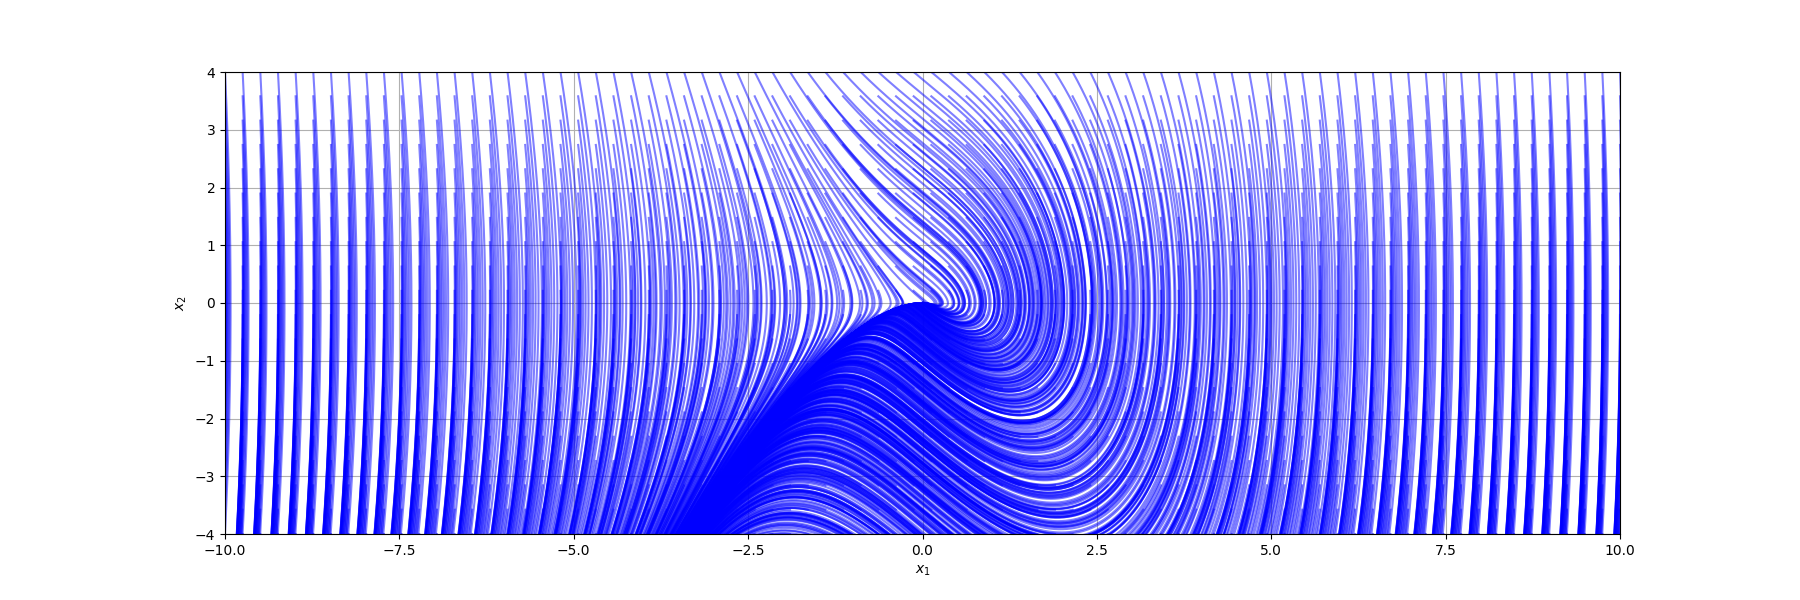
\includegraphics[width=\linewidth]{Images/nonlinear/introduction/phase.png}
    \caption{Phase portrait}
    \label{fig:phase}
\end{figure}
Consider the system
\begin{align}
    \dot{x}_1 &= x_2, \\
    \dot{x}_2 &= -x_1^2 - x_2.
\end{align}
\\
\textbf{Step 1: Equilibrium Points.}  
\\Solve
\[
x_2 = 0, \qquad -x_1^2 - x_2 = 0.
\]
This gives the only equilibrium at $(x_1, x_2) = (0,0)$.
\\\\
\textbf{Step 2: Vector Field.}  
\\The vector field in the $(x_1,x_2)$ plane is obtained (as shown in figure \ref{fig:phase}) by evaluating
\[
\dot{x}_1 = x_2, \qquad \dot{x}_2 = -x_1^2 - x_2.
\]


\textbf{Observation.}  
- The equilibrium at $(0,0)$ is asymptotically stable, since $x_2$ introduces damping and $-x_1^2$ is always nonpositive.  
- Trajectories spiral or curve toward the origin but with nonlinear effects due to the $-x_1^2$ term.
\end{example}

\section{Phase-Plane Analysis of LTI Systems}\index{Phase-Plane Analysis of LTI Systems}

We now specialize phase-plane analysis to \emph{linear time-invariant (LTI)} systems of the form
\begin{equation}
    \dot{x}(t) = A x(t), \qquad A \in \mathbb{R}^{2\times 2}.
\end{equation}
The solution is
\begin{equation}
    x(t) = e^{At} x(0).
\end{equation}
The qualitative behavior depends only on the eigenvalues of $A$.  

\subsection{Case 1: Diagonalizable Systems with Real Eigenvalues}\index{Phase-Plane Analysis of LTI Systems!Case 1}

Suppose $A$ has two distinct real eigenvalues $\lambda_1, \lambda_2$ with corresponding linearly independent eigenvectors $v_1, v_2$.  
Then, $A$ is diagonalizable:
\[
A = T D T^{-1}, \qquad D = \text{diag}(\lambda_1,\lambda_2),
\]
so that in the transformed coordinates $z = T^{-1}x$,
\[
\dot{z} = Dz =
\begin{bmatrix}
\lambda_1 & 0 \\
0 & \lambda_2
\end{bmatrix} z.
\]

The solutions are
\[
z_1(t) = z_1(0)e^{\lambda_1 t}, \qquad z_2(t) = z_2(0)e^{\lambda_2 t}.
\]

\paragraph{Qualitative Behavior.}
\begin{itemize}
    \item If $\lambda_1, \lambda_2 < 0$: trajectories decay to the origin (stable node).
    \item If $\lambda_1, \lambda_2 > 0$: trajectories diverge (unstable node).
    \item If $\lambda_1 \lambda_2 < 0$: trajectories approach along the stable direction and diverge along the unstable one (saddle point).
\end{itemize}

The eigenvectors define the principal axes of trajectories in the phase plane.

\subsection{Case 2: Non-Diagonalizable Systems (Defective Matrix)}\index{Phase-Plane Analysis of LTI Systems!Case 2}

If $A$ has a repeated eigenvalue $\lambda$ but only one independent eigenvector, then it is not diagonalizable.  
Instead, we form the Jordan form:
\[
A = P J P^{-1}, \qquad J =
\begin{bmatrix}
\lambda & 1 \\
0 & \lambda
\end{bmatrix}.
\]

The solution in Jordan coordinates is
\[
z(t) =
\begin{bmatrix}
e^{\lambda t} & t e^{\lambda t} \\
0 & e^{\lambda t}
\end{bmatrix} z(0).
\]

\paragraph{Qualitative Behavior.}
\begin{itemize}
    \item If $\lambda < 0$: trajectories decay to the origin but not along straight lines; they are distorted due to the $t e^{\lambda t}$ term.
    \item If $\lambda > 0$: trajectories diverge with polynomially growing components.
    \item If $\lambda = 0$: trajectories grow linearly with $t$ (marginal stability).
\end{itemize}

In the phase plane, trajectories are tangent to the single eigenvector direction but curve due to the generalized eigenvector contribution.

\subsection{Case 3: Systems with Complex Eigenvalues}\index{Phase-Plane Analysis of LTI Systems!Case 3}

If $A$ has complex-conjugate eigenvalues $\lambda_{1,2} = \alpha \pm j\beta$ with $\beta \neq 0$, then $A$ can be transformed into
\[
M^{-1} A M =
\begin{bmatrix}
\alpha & -\beta \\
\beta & \alpha
\end{bmatrix}.
\]

The solution is
\[
z(t) = e^{\alpha t}
\begin{bmatrix}
\cos(\beta t) & -\sin(\beta t) \\
\sin(\beta t) & \cos(\beta t)
\end{bmatrix} z(0).
\]

\paragraph{Qualitative Behavior.}
\begin{itemize}
    \item If $\alpha < 0$: trajectories spiral into the origin (stable focus).
    \item If $\alpha > 0$: trajectories spiral outward (unstable focus).
    \item If $\alpha = 0$: trajectories form closed orbits (center, neutrally stable).
\end{itemize}

The frequency of oscillation is $\beta$, and $\alpha$ determines whether the spiral converges or diverges.

\begin{example}[Comparison of LTI Systems]
\begin{figure}[h!]
    \centering
    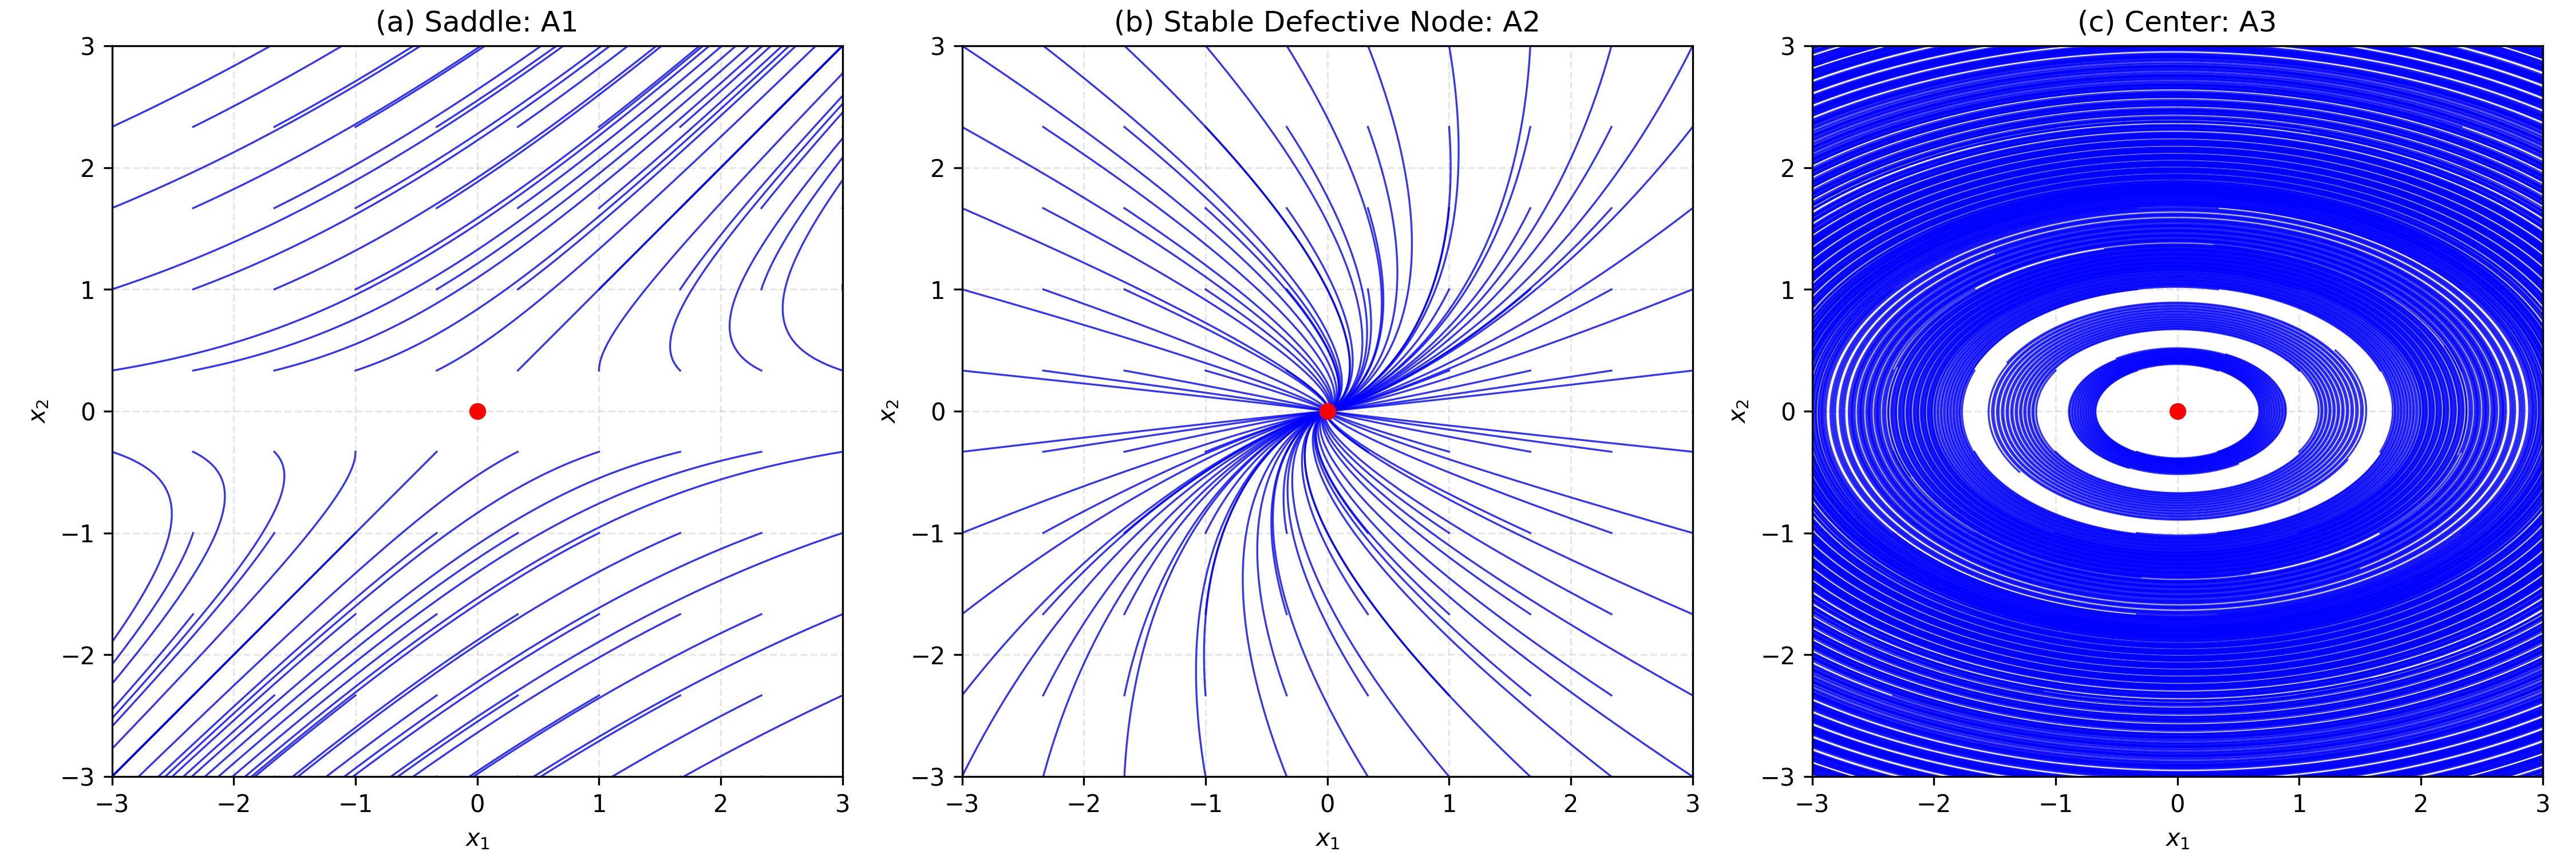
\includegraphics[width=\linewidth]{Images/nonlinear/introduction/phase_dense.png}
    \caption{Phase portraits of three different LTI systems: 
    (a) saddle point, 
    (b) stable defective node, 
    (c) center.}
    \label{fig:lti_phase}
\end{figure}

We compare the qualitative behavior of three linear time-invariant systems of the form
\[
\dot{x}(t) = A x(t), \qquad A \in \mathbb{R}^{2\times 2}.
\]

\textbf{Case 1: Saddle Point.}  
\[
A_1 = \begin{bmatrix} -1 & 3 \\ 0 & 2 \end{bmatrix}.
\]
Eigenvalues are $\lambda_1=-1$, $\lambda_2=2$ with opposite signs.  
Trajectories approach the origin along the stable direction and diverge along the unstable one, forming a saddle (Fig.~\ref{fig:lti_phase}a).

\textbf{Case 2: Stable Defective Node.}  
\[
A_2 = \begin{bmatrix} -2 & 1 \\ 0 & -2 \end{bmatrix}.
\]
This has a repeated eigenvalue $\lambda=-2$ with only one eigenvector.  
Trajectories converge to the origin but are distorted due to the Jordan block structure, curving toward the equilibrium (Fig.~\ref{fig:lti_phase}b).

\textbf{Case 3: Center.}  
\[
A_3 = \begin{bmatrix} 0 & -3 \\ 1 & 0 \end{bmatrix}.
\]
Eigenvalues are purely imaginary $\lambda = \pm j\sqrt{3}$.  
Trajectories form closed orbits, indicating a neutrally stable center (Fig.~\ref{fig:lti_phase}c).
\end{example}

\subsection{Conclusion}\index{Phase-Plane Analysis of LTI Systems!Conclusion}
\begin{table}[h!]
    \centering
    \begin{tabular}{|c|c|}\hline
         \textbf{Eigenvalues} & \textbf{Equilibrium type} \\\hline
         $\lambda_1,\lambda_2$ real, both $<0$ & Stable node \\\hline
         $\lambda_1,\lambda_2$ real, both $>0$ & Unstable node \\\hline
         $\lambda_1\lambda_2 < 0$ (real, opposite signs) & Saddle point \\\hline
         Complex with $\Re(\lambda)<0$ & Stable focus (spiral in) \\\hline
         Complex with $\Re(\lambda)>0$ & Unstable focus (spiral out) \\\hline
         Purely imaginary ($\Re(\lambda)=0$) & Center (neutrally stable) \\\hline
    \end{tabular}
    \caption{Summary of different equilibrium cases for $2\times2$ LTI systems.}
    \label{tab:lti_summary}
\end{table}

\section{Phase Plane Analysis of Nonlinear Systems}\index{Phase Plane Analysis of Nonlinear Systems}

Unlike linear systems, nonlinear systems often exhibit phenomena such as 
\emph{self-excited oscillations}. These oscillations do not require external forcing
and are called \textbf{limit cycles}. A limit cycle is a closed trajectory in the 
phase plane that is isolated, meaning nearby trajectories either spiral towards it 
(stable) or away from it (unstable). 

\subsection{Limit Cycles}\index{Phase Plane Analysis of Nonlinear Systems!Limit Cycles}

One of the most famous examples of a system with a limit cycle is the 
\textbf{Van der Pol oscillator}.

\begin{definition}[Van der Pol Oscillator]
    The Van der Pol oscillator is governed by the second-order nonlinear differential equation
    \begin{equation}
        \ddot{x} - \mu(1-x^2)\dot{x} + x = 0, \qquad \mu \geq 0
    \end{equation}
    where $\mu$ is a scalar parameter controlling nonlinearity and damping.
\end{definition}

\subsubsection*{State-Space Form}
Let $x_1 = x$ and $x_2 = \dot{x}$, then
\begin{align}
    \dot{x}_1 &= x_2 \\
    \dot{x}_2 &= \mu(1 - x_1^2)x_2 - x_1
\end{align}
This defines the nonlinear vector field:
\[
\dot{\mathbf{x}} =
\begin{bmatrix}
x_2 \\
\mu(1-x_1^2)x_2 - x_1
\end{bmatrix}.
\]

\subsubsection*{Equilibrium and Dynamics}
\begin{remark}
    For $\mu = 0$, the system reduces to the linear oscillator
    \begin{equation}
        \dot{x}_1 = x_2, \qquad \dot{x}_2 = -x_1,
    \end{equation}
    which has the origin $(0,0)$ as a center with closed trajectories (neutrally stable).
\end{remark}

\begin{remark}
    For $\mu > 0$, the nonlinear term $\mu(1-x_1^2)x_2$ introduces:
    \begin{itemize}
        \item Negative damping near the origin, pushing trajectories outward.
        \item Positive damping for large $|x_1|$, pulling trajectories inward.
    \end{itemize}
    This balance creates a \textbf{stable limit cycle}, i.e. all trajectories converge to a periodic orbit.
\end{remark}

\begin{example}[Vector Field of Van der Pol Oscillator: Stable vs. Unstable]
    The Van der Pol oscillator in state-space form is
    \begin{align}
        \dot{x}_1 &= x_2 \\
        \dot{x}_2 &= \pm \mu (1-x_1^2)x_2 - x_1,
    \end{align}
    where the choice of sign determines the nature of the dynamics:
    \begin{itemize}
        \item With $+\mu$, the system exhibits a \textbf{stable limit cycle}, attracting trajectories.  
        \item With $-\mu$, the system exhibits an \textbf{unstable limit cycle}, repelling trajectories.  
    \end{itemize}

    The corresponding vector fields for $\mu=1$ are shown below.

    \begin{figure}[h!]
        \centering
        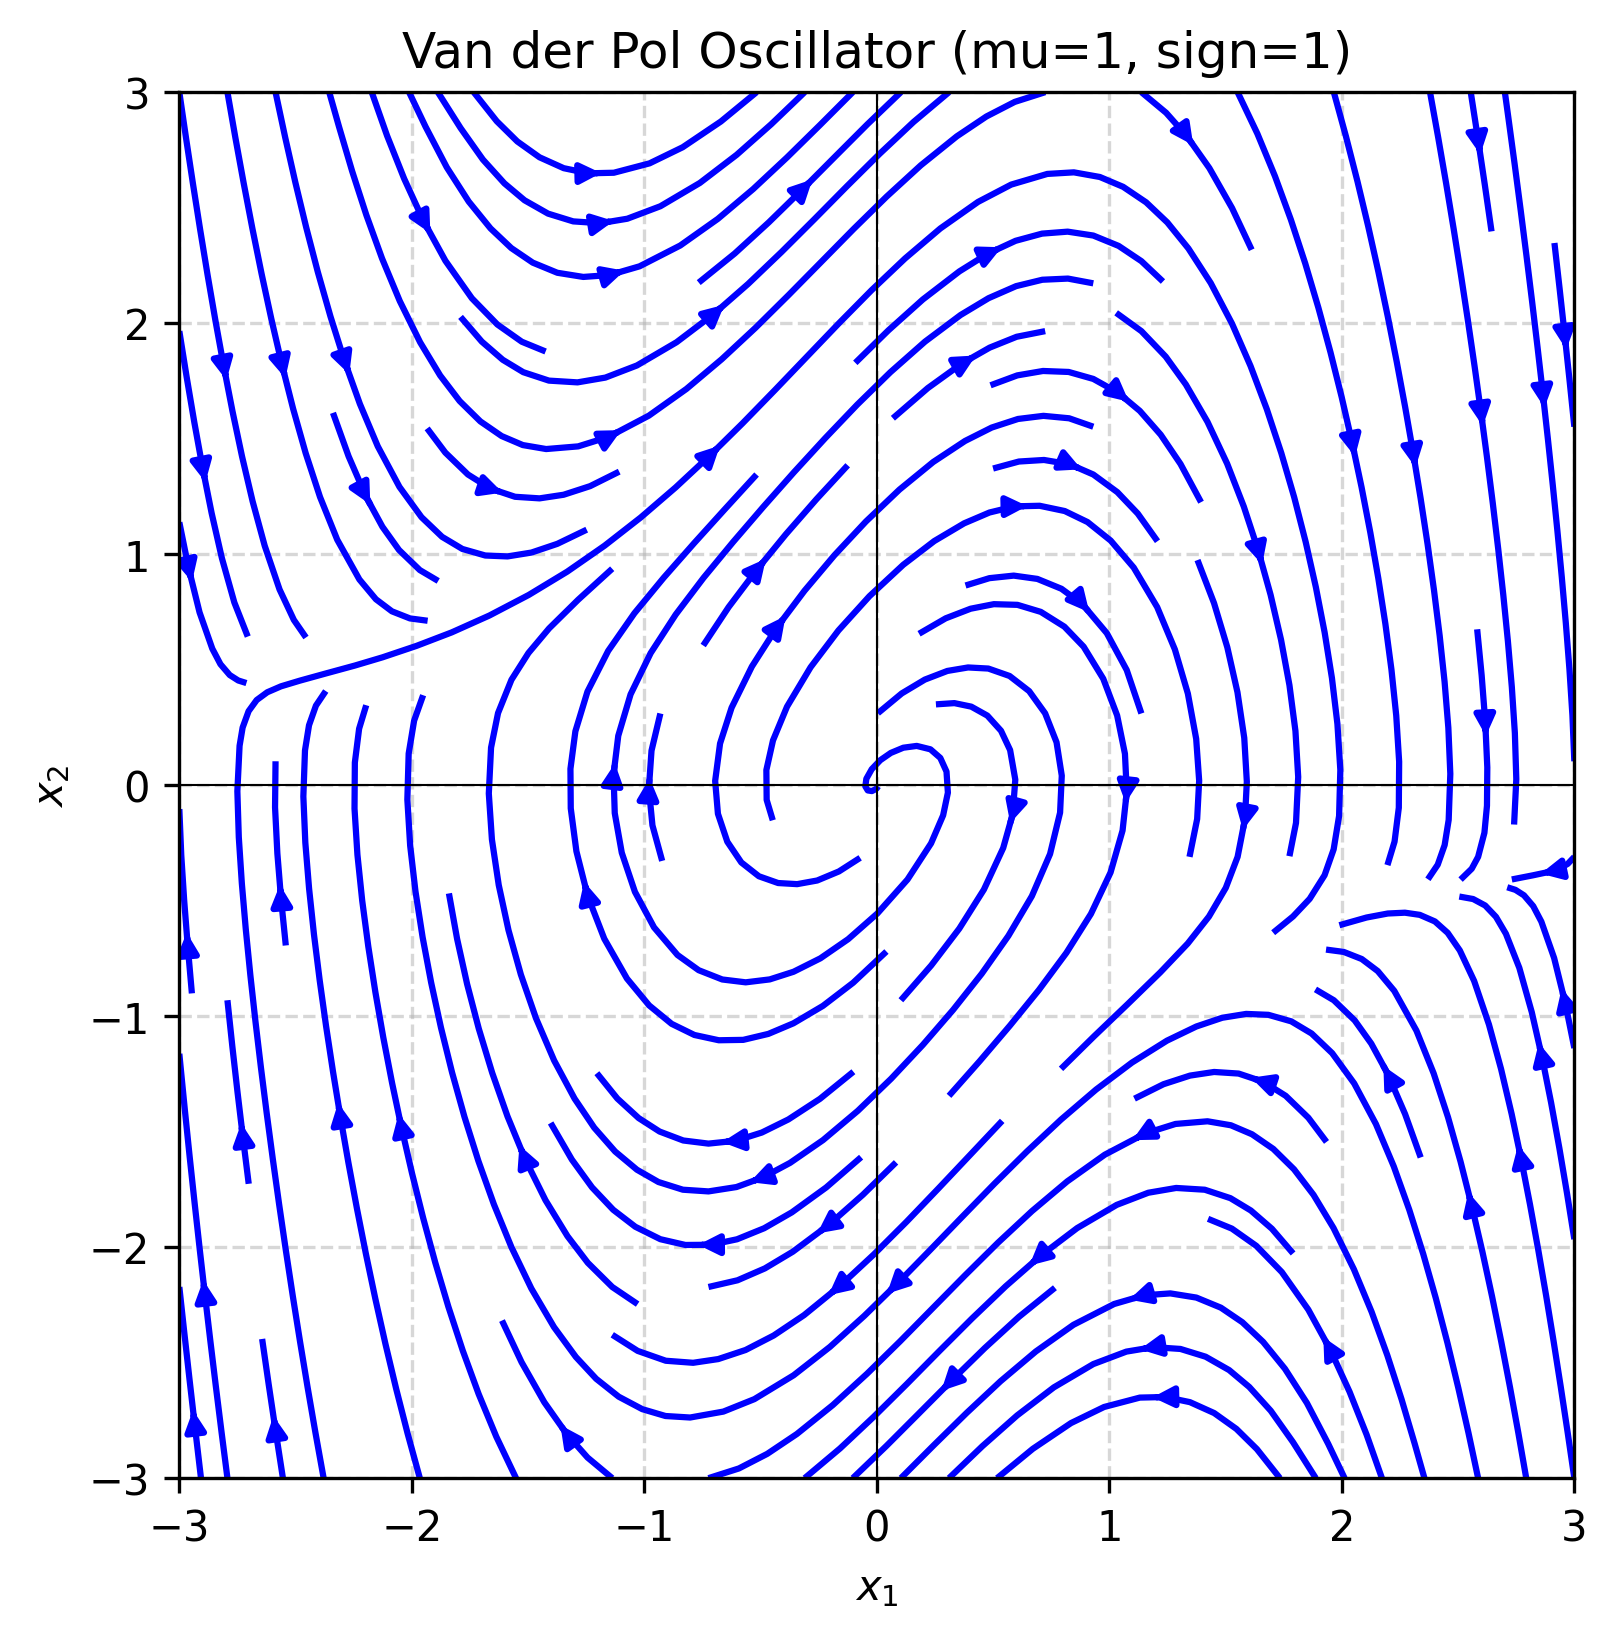
\includegraphics[width=0.4\textwidth]{Images/nonlinear/introduction/vdp_stable.png}
        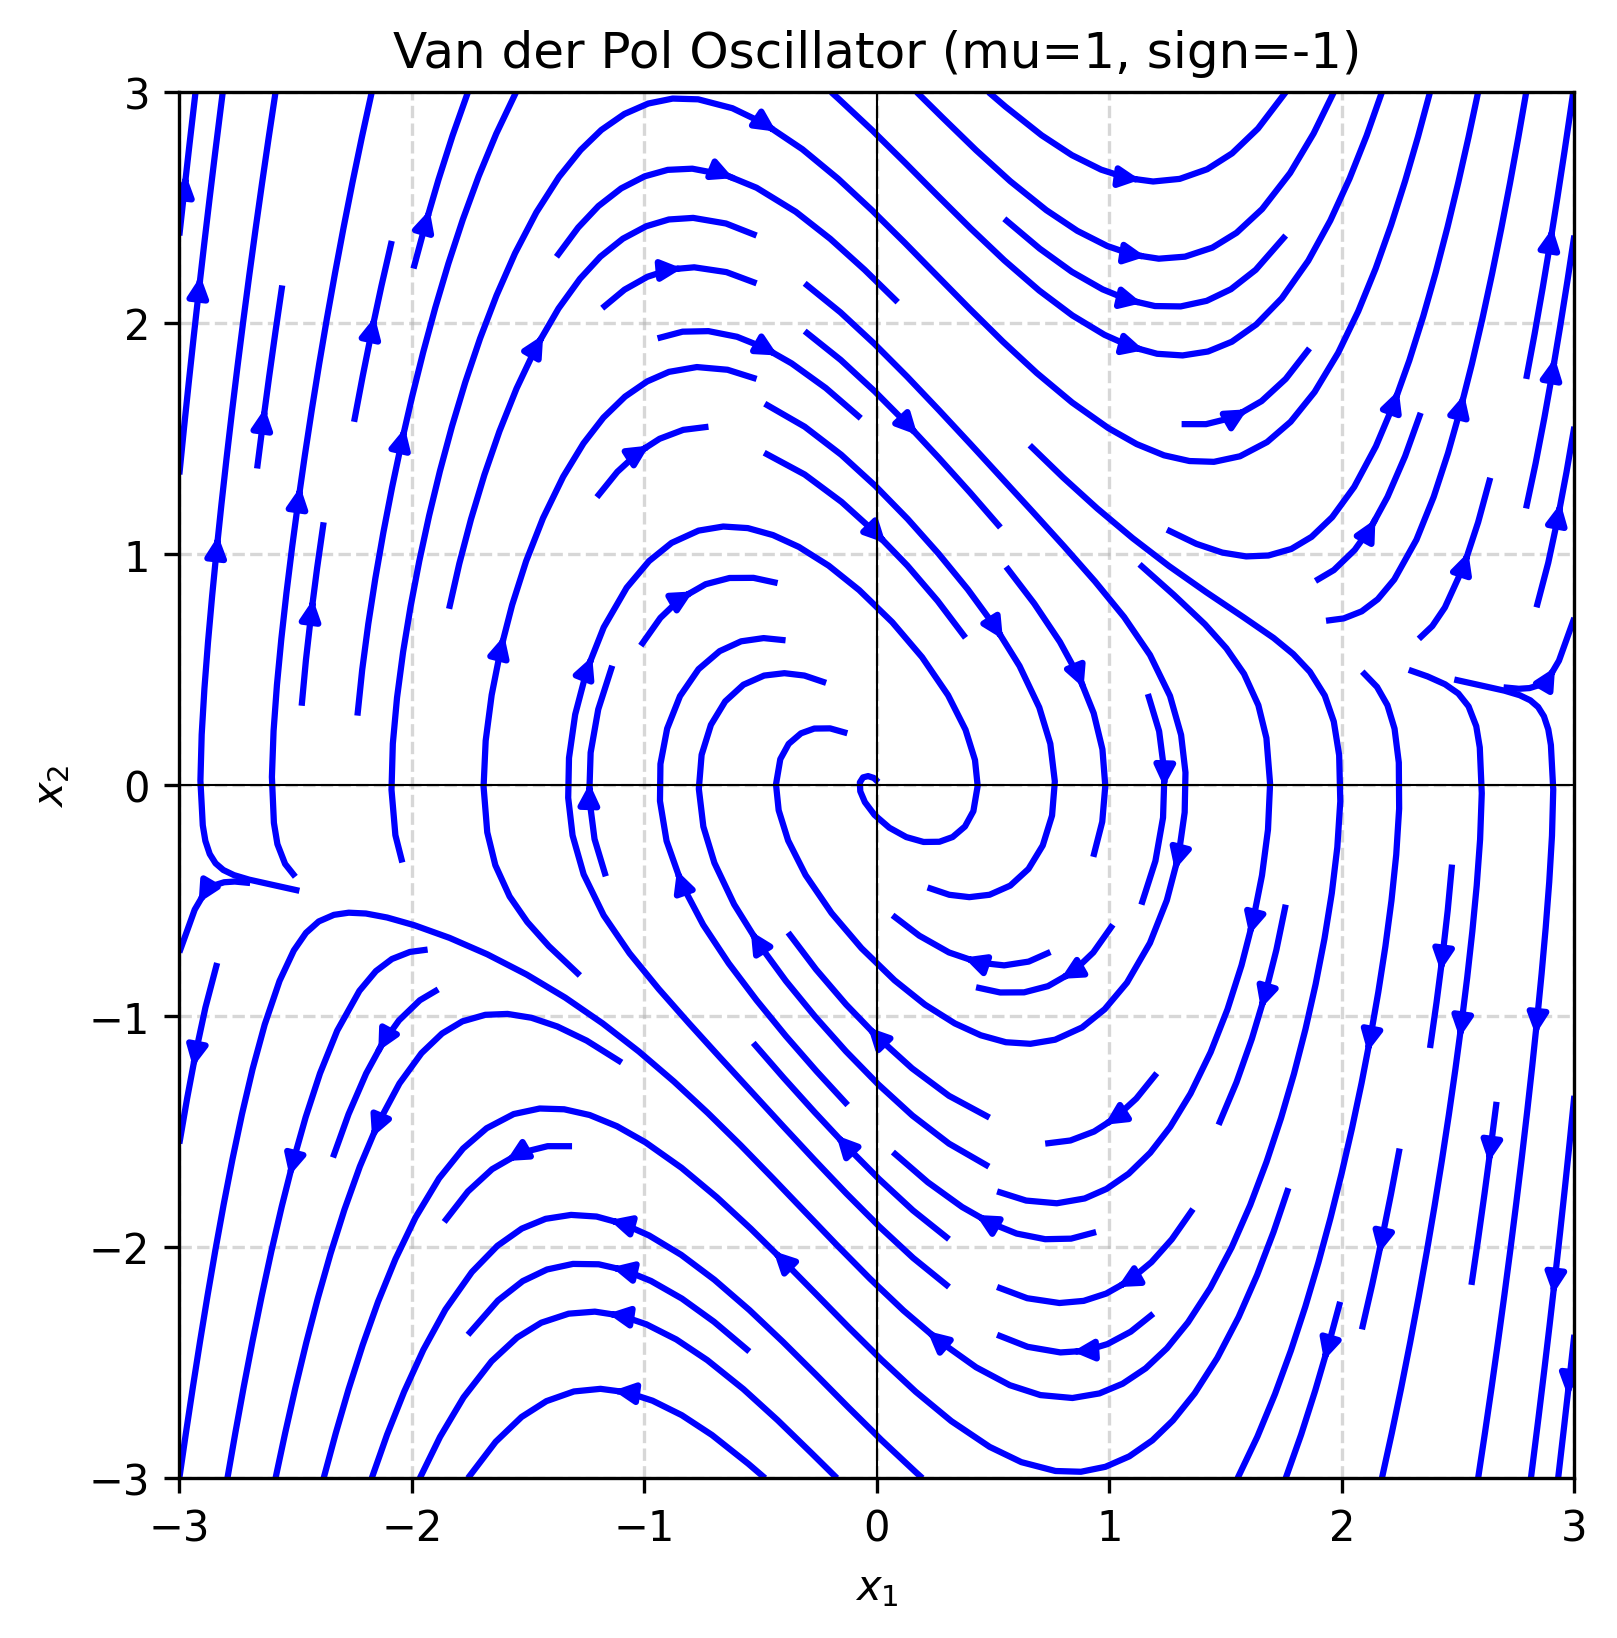
\includegraphics[width=0.4\textwidth]{Images/nonlinear/introduction/vdp_unstable.png}
        \caption{Phase portraits of the Van der Pol oscillator for $\mu=1$: stable limit cycle (left) and unstable limit cycle (right).}
    \end{figure}
\end{example}


\begin{remark}
A \textbf{stable limit cycle} attracts nearby trajectories, an \textbf{unstable limit cycle} repels them, and a \textbf{semistable limit cycle} attracts trajectories on one side while repelling on the other. 
\end{remark}


\chapterimage{orange2.jpg} % Chapter heading image
\chapterspaceabove{6.75cm} % Whitespace from the top of the page to the chapter title on chapter pages
\chapterspacebelow{7.25cm} % Amount of vertical whitespace from the top margin to the start of the text on chapter pages

\chapter{Mathematical Preliminaries}\index{Mathematical Preliminaries}
\section{Overview}\index{Overview}
In this chapter, we introduce key mathematical tools that will be used throughout the book, such as matrices, vector spaces, norms, and inner products. These concepts provide the foundation for analyzing systems, describing their behavior, and formulating methods for control and stability. Our focus will be on essential definitions, properties, and operations, presented in a clear and application-oriented manner. The aim is to build a working knowledge of these preliminaries that can be readily applied in the upcoming chapters.


\section{Sets}\index{Sets}

\begin{definition}[Set]
A \emph{set} is a well-defined collection of distinct objects, considered as an object in its own right. The objects in a set are called its \emph{elements} or \emph{members}, and if $x$ is an element of a set $A$, we write $x \in A$. 
\end{definition}

\begin{notation}
Commonly used notations for sets include:
\begin{itemize}
    \item $\mathbb{N}$: Natural numbers $\{1,2,3,\dots\}$
    \item $\mathbb{Z}$: Integers $\{\dots,-2,-1,0,1,2,\dots\}$
    \item $\mathbb{Q}$: Rational numbers
    \item $\mathbb{R}$: Real numbers
    \item $\mathbb{C}$: Complex numbers
\end{itemize}
\end{notation}

\begin{example}[Set Operations]
Let $A = \{1,2,3,4\}$ and $B = \{3,4,5,6\}$.  
\begin{itemize}
    \item Union: $A \cup B = \{1,2,3,4,5,6\}$  
    \item Intersection: $A \cap B = \{3,4\}$  
    \item Difference: $A \setminus B = \{1,2\}$  
    \item Cartesian Product: $A \times B = \{(a,b)\,|\, a \in A, b \in B\}$  
\end{itemize}
\end{example}

\begin{remark}
Sets may be finite or infinite. Infinite sets such as $\mathbb{N}$ and $\mathbb{R}$ play a central role in mathematics, especially in analysis and control theory.
\end{remark}

%------------------------------------------------
\section{Metric Spaces}\index{Metric Spaces}

\begin{definition}[Metric Space]
A \emph{metric space} is a pair $(X,d)$ where $X$ is a non-empty set and 
$d : X \times X \to \mathbb{R}$ is a function, called a \emph{metric}, such that for all $x,y,z \in X$:
\begin{align}
    & d(x,y) \geq 0 \quad \text{(non-negativity)} \\
    & d(x,y) = 0 \iff x=y \quad \text{(identity of indiscernibles)} \\
    & d(x,y) = d(y,x) \quad \text{(symmetry)} \\
    & d(x,z) \leq d(x,y) + d(y,z) \quad \text{(triangle inequality)}
\end{align}
\end{definition}

\begin{notation}
Commonly used metrics include:
\begin{itemize}
    \item Euclidean metric: $d(x,y) = \|x-y\|_2$ on $\mathbb{R}^n$  
    \item Manhattan metric: $d(x,y) = \|x-y\|_1 = \sum |x_i - y_i|$  
    \item Maximum metric: $d(x,y) = \|x-y\|_\infty = \max |x_i - y_i|$  
\end{itemize}
\end{notation}

\begin{example}
Let $X = \mathbb{R}^2$ and define $d(x,y) = \sqrt{(x_1-y_1)^2+(x_2-y_2)^2}$.  
Then $(\mathbb{R}^2,d)$ is a metric space with the standard Euclidean distance.
\end{example}

\begin{remark}
Every normed vector space $(V,\|\cdot\|)$ induces a metric by defining $d(x,y) = \|x-y\|$.  
Thus, metric spaces generalize the familiar notion of distance while allowing greater flexibility in analysis.
\end{remark}

%------------------------------------------------
\section{Vector Spaces}\index{Vector Spaces}

\begin{definition}[Vector Space]
A \emph{vector space} $V$ over a field $\mathbb{K}$ (where $\mathbb{K} = \mathbb{R}$ or $\mathbb{C}$) is a non-empty set together with two operations:
\begin{itemize}
    \item \textbf{Vector addition:} $+\ : V \times V \to V$
    \item \textbf{Scalar multiplication:} $\cdot\ : \mathbb{K} \times V \to V$
\end{itemize}
such that the usual axioms of associativity, commutativity, distributivity, and existence of additive identity and inverse hold.
\end{definition}

\begin{example}
The set $\mathbb{R}^n$ with componentwise addition and scalar multiplication is a vector space over $\mathbb{R}$.  
For instance, in $\mathbb{R}^2$:  
\[
(x_1,x_2) + (y_1,y_2) = (x_1+y_1,\; x_2+y_2), \quad 
\lambda(x_1,x_2) = (\lambda x_1,\; \lambda x_2).
\]
\end{example}

%------------------------------------------------
\subsection{Linear Independence and Basis}\index{Vector Spaces!Linear Independence and Basis}

\begin{definition}[Linear Independence]
A set of vectors $\{v_1,v_2,\dots,v_k\}$ in $V$ is said to be \emph{linearly independent} if 
\[
\alpha_1 v_1 + \alpha_2 v_2 + \cdots + \alpha_k v_k = 0 \quad \Rightarrow \quad \alpha_1=\alpha_2=\cdots=\alpha_k=0.
\]
Otherwise, the set is \emph{linearly dependent}.
\end{definition}

\begin{definition}[Basis and Dimension]
A \emph{basis} of a vector space $V$ is a linearly independent set of vectors that spans $V$.  
The number of elements in a basis is called the \emph{dimension} of $V$, denoted $\dim(V)$.
\end{definition}

\begin{theorem}
In $\mathbb{R}^n$, any set of $n+1$ or more vectors is linearly dependent.
\end{theorem}

\begin{example}
In $\mathbb{R}^3$, the vectors $e_1=(1,0,0)$, $e_2=(0,1,0)$, and $e_3=(0,0,1)$ form a basis.  
They are linearly independent, and every vector $(x,y,z) \in \mathbb{R}^3$ can be written uniquely as 
\[
(x,y,z) = x e_1 + y e_2 + z e_3.
\]
Hence, $\dim(\mathbb{R}^3)=3$.
\end{example}

%------------------------------------------------
\subsection{Subspaces}\index{Vector Spaces!Subspaces}

\begin{definition}[Subspace]
A subset $W \subseteq V$ is called a \emph{subspace} of $V$ if:
\begin{itemize}
    \item $0 \in W$,
    \item $u,v \in W \Rightarrow u+v \in W$,
    \item $u \in W, \lambda \in \mathbb{K} \Rightarrow \lambda u \in W$.
\end{itemize}
\end{definition}

\begin{definition}[Span]
Given a set of vectors $S = \{v_1,\dots,v_k\}$ in $V$, the \emph{span} of $S$, denoted $\mathrm{span}(S)$, is the set of all linear combinations of the vectors in $S$.  
That is, 
\[
\mathrm{span}(S) = \Big\{ \sum_{i=1}^k \alpha_i v_i \; : \; \alpha_i \in \mathbb{K} \Big\}.
\]
\end{definition}

\begin{example}
In $\mathbb{R}^3$, let $S=\{(1,0,0), (0,1,0)\}$.  
The span of $S$ is 
\[
\mathrm{span}(S) = \{(x,y,0) \in \mathbb{R}^3 \mid x,y \in \mathbb{R}\},
\]
which is a subspace of $\mathbb{R}^3$ corresponding to the $xy$-plane.
\end{example}

%------------------------------------------------
\subsection{Normed Vector Spaces}\index{Vector Spaces!Normed Vector Spaces}

\begin{definition}[Normed Vector Space]
A \emph{normed vector space} is a pair $(V,\|\cdot\|)$ where $V$ is a vector space and $\|\cdot\|: V \to \mathbb{R}$ satisfies, for all $x,y \in V$ and $\lambda \in \mathbb{K}$:
\begin{align}
& \|x\| \geq 0, \quad \|x\| = 0 \iff x=0 \quad \text{(positivity)} \\
& \|\lambda x\| = |\lambda| \|x\| \quad \text{(homogeneity)} \\
& \|x+y\| \leq \|x\| + \|y\| \quad \text{(triangle inequality)}
\end{align}
\end{definition}

\begin{theorem}[Hölder's Inequality]
For $x,y \in \mathbb{R}^n$ and $p,q > 1$ with $\tfrac{1}{p}+\tfrac{1}{q}=1$,  
\[
\sum_{i=1}^n |x_i y_i| \;\leq\; \left( \sum_{i=1}^n |x_i|^p \right)^{1/p} 
\left( \sum_{i=1}^n |y_i|^q \right)^{1/q}.
\]
\end{theorem}

\begin{theorem}[Minkowski's Inequality]
For $x,y \in \mathbb{R}^n$ and $p \geq 1$,  
\[
\left( \sum_{i=1}^n |x_i+y_i|^p \right)^{1/p} \;\leq\; 
\left( \sum_{i=1}^n |x_i|^p \right)^{1/p} + 
\left( \sum_{i=1}^n |y_i|^p \right)^{1/p}.
\]
\end{theorem}

\begin{example}
Consider $V=\mathbb{R}^2$ with the Euclidean norm $\|(x,y)\|_2=\sqrt{x^2+y^2}$.  
Then $(\mathbb{R}^2,\|\cdot\|_2)$ is a normed vector space.  
For example, $\|(3,4)\|_2=\sqrt{3^2+4^2}=5$.
\end{example}

%------------------------------------------------
\section{Matrices}\index{Matrices}

\subsection{Basic Properties}\index{Matrices!Basic Properties}

\begin{itemize}
    \item \textbf{Transpose:} For a matrix $A=(a_{ij}) \in \mathbb{R}^{m \times n}$, the transpose is $A^T=(a_{ji}) \in \mathbb{R}^{n \times m}$.  
    Properties:
    \begin{align*}
        (A^T)^T &= A, \\
        (A+B)^T &= A^T + B^T, \\
        (\alpha A)^T &= \alpha A^T, \quad \alpha \in \mathbb{R}, \\
        (AB)^T &= B^T A^T.
    \end{align*}
    
    \item \textbf{Symmetric Matrix:} $A \in \mathbb{R}^{n \times n}$ is symmetric if $A^T = A$.

    \item \textbf{Skew-Symmetric Matrix:} $A \in \mathbb{R}^{n \times n}$ is skew-symmetric if $A^T = -A$.

    \item \textbf{Orthogonal Matrix:} $A \in \mathbb{R}^{n \times n}$ is orthogonal if $A^T A = I$.  
    In this case, $A^{-1} = A^T$.

    \item \textbf{Inverse:} A square matrix $A$ is invertible (or nonsingular) if there exists $A^{-1}$ such that $AA^{-1}=A^{-1}A=I$.

    \item \textbf{Rank:} The rank of a matrix $A$, denoted $\mathrm{rank}(A)$, is the dimension of the column space (or row space) of $A$.
\end{itemize}

\begin{definition}[Null Space]
The \emph{null space} (or kernel) of $A \in \mathbb{R}^{m \times n}$ is
\[
\mathcal{N}(A) = \{x \in \mathbb{R}^n \mid Ax = 0\}.
\]
\end{definition}

\begin{theorem}[Rank-Nullity Theorem]
For $A \in \mathbb{R}^{m \times n}$,  
\[
\mathrm{rank}(A) + \dim(\mathcal{N}(A)) = n.
\]
\end{theorem}

%------------------------------------------------
\subsection{Eigenvalues, Eigenvectors and Diagonalization}\index{Matrices!Eigenvalues and Eigenvectors}

\begin{definition}[Eigenvalue and Eigenvector]
For a square matrix $A \in \mathbb{R}^{n \times n}$, a nonzero vector $v \in \mathbb{R}^n$ is an \emph{eigenvector} if 
\[
Av = \lambda v
\]
for some scalar $\lambda \in \mathbb{R}$, called an \emph{eigenvalue}.
\end{definition}

\begin{theorem}[Diagonalization]
If $A \in \mathbb{R}^{n \times n}$ has $n$ linearly independent eigenvectors, then $A$ is diagonalizable, i.e.,
\[
A = S D S^{-1},
\]
where $D$ is diagonal with the eigenvalues of $A$ on its diagonal, and $S$ is the matrix of eigenvectors.
\end{theorem}

\begin{theorem}[Special Case: Symmetric Matrices]
If $A \in \mathbb{R}^{n \times n}$ is real and symmetric, then:
\begin{itemize}
    \item All eigenvalues of $A$ are real.
    \item $A$ admits an orthogonal diagonalization: $A = Q D Q^T$, where $Q$ is orthogonal and $D$ diagonal.
\end{itemize}
\end{theorem}

%------------------------------------------------
\subsection{Quadratic Forms}\index{Matrices!Quadratic Forms}

A quadratic form on $\mathbb{R}^n$ associated with a matrix $A \in \mathbb{R}^{n \times n}$ is
\[
q(x) = x^T A x, \quad x \in \mathbb{R}^n.
\]
Without loss of generality, $A$ can be assumed symmetric.

\begin{definition}[Definiteness of Quadratic Forms]
Let $q(x) = x^T A x$, with $A$ symmetric.
\begin{itemize}
    \item $q$ is \textbf{positive definite} if $q(x) > 0$ for all $x \neq 0$.
    \item $q$ is \textbf{positive semidefinite} if $q(x) \geq 0$ for all $x$.
    \item $q$ is \textbf{negative definite} if $q(x) < 0$ for all $x \neq 0$.
    \item $q$ is \textbf{negative definite} if $q(x) \leq 0$ for all $x \neq 0$.
    \item $q$ is \textbf{indefinite} if it takes both positive and negative values.
\end{itemize}
\end{definition}

\begin{theorem}[Rayleigh’s Inequality]
For a symmetric matrix $A \in \mathbb{R}^{n \times n}$ with eigenvalues $\lambda_{\min} \leq \cdots \leq \lambda_{\max}$,  
the Rayleigh quotient
\[
R(x) = \frac{x^T A x}{x^T x}, \quad x \neq 0,
\]
satisfies
\[
\lambda_{\min} \leq R(x) \leq \lambda_{\max}.
\]
\end{theorem}

%------------------------------------------------
\section{Basic Topology}\index{Topology}

\subsection{Topology in Metric Spaces}\index{Topology!Metric Spaces}

Let $(X,d)$ be a metric space. We introduce the following concepts:

\begin{itemize}
    \item \textbf{Neighborhood:} A set $N_\epsilon(x) = \{y \in X : d(x,y) < \epsilon\}$ is called an $\epsilon$-neighborhood of $x \in X$.

    \item \textbf{Limit Point:} A point $x \in X$ is a limit point of a set $A \subseteq X$ if every neighborhood of $x$ contains a point of $A$ other than $x$ itself.

    \item \textbf{Interior Point:} A point $x \in A \subseteq X$ is an interior point of $A$ if there exists $\epsilon > 0$ such that $N_\epsilon(x) \subseteq A$.

    \item \textbf{Open Set:} A set $A \subseteq X$ is open if every point of $A$ is an interior point of $A$.

    \item \textbf{Complement:} The complement of $A \subseteq X$ is $A^c = X \setminus A$.

    \item \textbf{Closed Set:} A set $A \subseteq X$ is closed if $A^c$ is open, or equivalently, if $A$ contains all its limit points.

    \item \textbf{Bounded Set:} A set $A \subseteq X$ is bounded if there exists $x \in X$ and $M > 0$ such that $d(x,y) \leq M$ for all $y \in A$.
\end{itemize}

%------------------------------------------------
\subsection{Basic Topology in $\mathbb{R}^n$}\index{Topology!Euclidean Space}

Let $\mathbb{R}^n$ be equipped with the Euclidean metric $d(x,y) = \|x-y\|_2$.  

\begin{itemize}
    \item \textbf{Subspace of $\mathbb{R}^n$:} Any subset $A \subseteq \mathbb{R}^n$ considered with the induced metric is called a subspace.

    \item \textbf{Neighborhood:} For $x \in \mathbb{R}^n$ and $\epsilon > 0$, the $\epsilon$-neighborhood is the open ball $B_\epsilon(x) = \{y \in \mathbb{R}^n : \|x-y\| < \epsilon\}$.

    \item \textbf{Open Set:} A set $A \subseteq \mathbb{R}^n$ is open if for every $x \in A$, there exists $\epsilon > 0$ such that $B_\epsilon(x) \subseteq A$.

    \item \textbf{Bounded Set:} $A \subseteq \mathbb{R}^n$ is bounded if it lies inside some ball $B_R(0)$ of finite radius $R > 0$.

    \item \textbf{Compact Set:} $A \subseteq \mathbb{R}^n$ is compact if it is closed and bounded (Heine–Borel theorem).

    \item \textbf{Convex Set:} $A \subseteq \mathbb{R}^n$ is convex if for any $x,y \in A$ and $\lambda \in [0,1]$, we have $\lambda x + (1-\lambda)y \in A$.
\end{itemize}

\section{Sequences}\index{Sequences}

\begin{definition}[Sequence of Vectors in a Metric Space]
A \emph{sequence} in a metric space $(X,d)$ is a function $\{x_n\}_{n=1}^\infty$ from the natural numbers $\mathbb{N}$ into $X$, i.e., a list of elements $x_1, x_2, x_3, \dots$ of $X$.
\end{definition}

\begin{definition}[Limit of a Sequence]
A sequence $\{x_n\}$ in a metric space $(X,d)$ is said to \emph{converge} to $x \in X$ if for every $\epsilon > 0$, there exists $N \in \mathbb{N}$ such that
\[
d(x_n, x) < \epsilon \quad \forall n \geq N.
\]
We then write $\lim_{n \to \infty} x_n = x$.
\end{definition}

\begin{example}[Convergent Sequence in $\mathbb{R}$]
In $(\mathbb{R}, |\cdot|)$, the sequence $x_n = \frac{1}{n}$ converges to $0$ because for any $\epsilon > 0$, if $n > \frac{1}{\epsilon}$ then $|x_n - 0| = \frac{1}{n} < \epsilon$.
\end{example}

\begin{example}[Sequence in $\mathbb{R}^2$]
In $(\mathbb{R}^2, \|\cdot\|_2)$, the sequence $x_n = \left(\frac{1}{n}, \frac{1}{n^2}\right)$ converges to $(0,0)$ because $\|x_n - (0,0)\|_2 = \sqrt{\frac{1}{n^2} + \frac{1}{n^4}} \to 0$ as $n \to \infty$.
\end{example}

\begin{definition}[Cauchy Sequence]
A sequence $\{x_n\}$ in a metric space $(X,d)$ is called a \emph{Cauchy sequence} if for every $\epsilon > 0$, there exists $N \in \mathbb{N}$ such that
\[
d(x_m, x_n) < \epsilon \quad \forall m,n \geq N.
\]
\end{definition}

\begin{example}[Cauchy Sequence in $\mathbb{Q}$]
Consider the sequence defined by the decimal approximations of $\sqrt{2}$: $x_1 = 1$, $x_2 = 1.4$, $x_3 = 1.41$, $x_4 = 1.414$, etc.  
This is a Cauchy sequence in $\mathbb{Q}$ because the terms get arbitrarily close, but it does \emph{not} converge in $\mathbb{Q}$ (it converges to $\sqrt{2} \notin \mathbb{Q}$).
\end{example}

\begin{definition}[Complete Metric Space]
A metric space $(X,d)$ is \emph{complete} if every Cauchy sequence in $X$ converges to a point in $X$.
\end{definition}

\begin{example}[Complete Space]
The metric space $(\mathbb{R}, |\cdot|)$ is complete: every Cauchy sequence of real numbers converges to a real number.  
In contrast, $(\mathbb{Q}, |\cdot|)$ is not complete, as shown by the sequence of rational approximations to $\sqrt{2}$.
\end{example}

\section{Functions}\index{Functions}

\begin{definition}[Function]
Let $A$ and $B$ be two sets.  
A \emph{function} $f$ from $A$ to $B$, denoted $f:A \to B$, is a rule that assigns to each $a \in A$ a unique element $b \in B$, written $f(a) = b$.  
\index{Function}
\end{definition}

\begin{example}
Consider $f:\mathbb{R} \to \mathbb{R}$ defined by $f(x) = x^2$.  
For each $x \in \mathbb{R}$, the function assigns a unique value $x^2 \in \mathbb{R}$.  
\end{example}

\begin{definition}[Composition of Functions]
Let $f:A \to B$ and $g:B \to C$ be two functions.  
The \emph{composition} of $g$ with $f$ is the function $g \circ f : A \to C$ defined by
\[
(g \circ f)(x) = g(f(x)), \qquad \forall x \in A.
\]
\index{Function!Composition}
\end{definition}

\begin{example}
Let $f:\mathbb{R}\to \mathbb{R}$ be $f(x)=x^2$, and $g:\mathbb{R}\to \mathbb{R}$ be $g(x)=\sin(x)$.  
Then $(g \circ f)(x) = \sin(x^2)$.  
\end{example}

\begin{definition}[Continuity in Metric Spaces]
Let $(X,d_X)$ and $(Y,d_Y)$ be metric spaces, and let $f:X \to Y$.  
The function $f$ is said to be \emph{continuous at} $x_0 \in X$ if for every $\epsilon > 0$, there exists $\delta > 0$ such that
\[
d_X(x,x_0) < \delta \;\;\Rightarrow\;\; d_Y(f(x), f(x_0)) < \epsilon.
\]
If $f$ is continuous at every point in $X$, then $f$ is called \emph{continuous on $X$}.  
\index{Continuity}
\end{definition}

\begin{example}
The function $f:\mathbb{R}\to \mathbb{R}$ defined by $f(x) = 3x+2$ is continuous everywhere since small changes in $x$ lead to proportionally small changes in $f(x)$.  
\end{example}

\begin{definition}[Uniform Continuity]
A function $f:X \to Y$ between metric spaces is called \emph{uniformly continuous} if for every $\epsilon > 0$, there exists $\delta > 0$ such that
\[
d_X(x_1,x_2) < \delta \;\;\Rightarrow\;\; d_Y(f(x_1), f(x_2)) < \epsilon
\]
for \emph{all} $x_1, x_2 \in X$.  
\index{Uniform Continuity}
\end{definition}

\begin{remark}
Continuity allows $\delta$ to depend on both $\epsilon$ and the point $x_0$.  
Uniform continuity requires a single $\delta$ (depending only on $\epsilon$) that works for the whole domain.  
\index{Continuity!Ordinary vs Uniform}
\end{remark}

\begin{example}
\begin{itemize}
    \item $f(x) = x^2$ is continuous on $\mathbb{R}$, but not uniformly continuous (as $x \to \infty$, the slope grows unbounded).  
    \item $f(x) = \sqrt{x}$ is uniformly continuous on $[0,\infty)$.  
\end{itemize}
\end{example}

\subsection{Bounded Linear Operators and Matrix Norms}\index{Functions!Bounded Linear Operators and Matrix Norms}

\begin{definition}[Linear Operator]
Let $X$ and $Y$ be vector spaces.  
A map $T:X \to Y$ is called a \emph{linear operator} if for all $x_1,x_2 \in X$ and scalars $\alpha,\beta \in \mathbb{R}$ (or $\mathbb{C}$),
\[
T(\alpha x_1 + \beta x_2) = \alpha T(x_1) + \beta T(x_2).
\]
\index{Operator!Linear}
\end{definition}

\begin{definition}[Bounded Linear Operator]
Let $(X,\|\cdot\|_X)$ and $(Y,\|\cdot\|_Y)$ be normed spaces.  
A linear operator $T:X \to Y$ is said to be \emph{bounded} if there exists $C>0$ such that
\[
\|Tx\|_Y \leq C \|x\|_X, \quad \forall x \in X.
\]
Equivalently, the \emph{operator norm} is defined as
\[
\|T\| = \sup_{x \neq 0} \frac{\|Tx\|_Y}{\|x\|_X} 
= \max_{\|x\|_X = 1} \|Tx\|_Y.
\]
\index{Operator!Bounded Linear}
\end{definition}

\begin{example}
Consider $T:\mathbb{R}^2 \to \mathbb{R}^2$ defined by $T(x,y) = (2x,3y)$.  
We compute:
\[
\|T(x,y)\|_\infty = \max(|2x|,|3y|).
\]
If $\|(x,y)\|_\infty = 1$, then the maximum value of $\|T(x,y)\|_\infty$ is $3$.  
Thus $\|T\|_\infty = 3$, and $T$ is bounded.  
\end{example}

\begin{definition}[Induced Matrix Norms]
Let $A \in \mathbb{R}^{n \times n}$.  
Given a vector norm $\|\cdot\|$ on $\mathbb{R}^n$, the \emph{induced matrix norm} is defined as
\[
\|A\| = \max_{\|x\|=1} \|Ax\|.
\]
\index{Matrix Norm}
\end{definition}

\begin{example}
For a matrix $A = (a_{ij}) \in \mathbb{R}^{n \times n}$, three common induced matrix norms are:
\begin{itemize}
    \item $\mathbf{1\text{-norm}}$:  
    \[
    \|A\|_1 = \max_{1 \leq j \leq n} \sum_{i=1}^n |a_{ij}| 
    \quad \text{(maximum absolute column sum)}.
    \]
    \item $\mathbf{\infty\text{-norm}}$:  
    \[
    \|A\|_\infty = \max_{1 \leq i \leq n} \sum_{j=1}^n |a_{ij}| 
    \quad \text{(maximum absolute row sum)}.
    \]
    \item $\mathbf{2\text{-norm}}$:  
    \[
    \|A\|_2 = \sqrt{\lambda_{\max}(A^TA)}
    \quad \text{(spectral norm)}.
    \]
\end{itemize}
\end{example}

\section{Differentiability}\index{Differentiaility}

\begin{definition}[Differentiability in $\mathbb{R}$]
A function $f:\mathbb{R}\to \mathbb{R}$ is said to be \emph{differentiable} at $x_0\in \mathbb{R}$ if the limit
\[
f'(x_0) = \lim_{h\to 0} \frac{f(x_0+h)-f(x_0)}{h}
\]
exists. The function $f'(x_0)$ is called the \emph{derivative} of $f$ at $x_0$.
\end{definition}

\begin{example}
The function $f(x)=x^2$ is differentiable everywhere with derivative $f'(x)=2x$.
\end{example}

\begin{example}
The function $f(x)=|x|$ is not differentiable at $x=0$, since the left and right limits of the difference quotient do not agree.
\end{example}


\begin{definition}[Differentiability in Higher Dimensions]
Let $f:\mathbb{R}^m\to \mathbb{R}^n$. We say $f$ is differentiable at $x_0\in \mathbb{R}^m$ if there exists a linear map 
$A:\mathbb{R}^m\to \mathbb{R}^n$ such that
\[
\lim_{h\to 0}\frac{\|f(x_0+h)-f(x_0)-A(h)\|}{\|h\|} = 0.
\]
The linear map $A$ is called the \emph{derivative} (or \emph{Jacobian matrix}) of $f$ at $x_0$.
\end{definition}

\begin{example}
Let $f:\mathbb{R}^2\to \mathbb{R}^2$ be given by $f(x,y)=(x^2+y,\, xy)$.  
Then 
\[
Df(x,y) = \begin{bmatrix}
2x & 1\\
y & x
\end{bmatrix}.
\]
\end{example}

\begin{definition}[Partial Derivative]
If $f:\mathbb{R}^m\to \mathbb{R}$, the \emph{partial derivative} with respect to $x_i$ at a point $x=(x_1,\dots,x_m)$ is
\[
\frac{\partial f}{\partial x_i}(x) = \lim_{h\to 0} \frac{f(x_1,\dots,x_i+h,\dots,x_m)-f(x)}{h}.
\]
\end{definition}

\begin{example}
For $f(x,y)=x^2y+e^y$, we have
\[
\frac{\partial f}{\partial x} = 2xy, \qquad \frac{\partial f}{\partial y} = x^2+e^y.
\]
\end{example}

\begin{definition}[Continuously Differentiable]
A function $f:\mathbb{R}^m\to \mathbb{R}^n$ is \emph{continuously differentiable} (denoted $C^1$) if it is differentiable and its derivative $Df(x)$ is continuous as a function of $x$.
\end{definition}

\begin{proposition}[Chain Rule]
Let $f:\mathbb{R}^m\to \mathbb{R}^n$ be differentiable at $x_0$, and $g:\mathbb{R}^n\to \mathbb{R}^p$ be differentiable at $f(x_0)$.  
Then $g\circ f:\mathbb{R}^m\to \mathbb{R}^p$ is differentiable at $x_0$, with
\[
D(g\circ f)(x_0) = Dg(f(x_0)) \cdot Df(x_0).
\]
\end{proposition}

\begin{example}
Let $f(x,y)=(x^2,y^2)$ and $g(u,v)=u+v$. Then $g\circ f(x,y)=x^2+y^2$.  
The chain rule gives
\[
D(g\circ f)(x,y)= [2x \quad 2y],
\]
which matches the direct derivative.
\end{example}

\begin{theorem}[Mean Value Theorem]
If $f:[a,b]\to \mathbb{R}$ is continuous on $[a,b]$ and differentiable on $(a,b)$, then there exists $c\in (a,b)$ such that
\[
f'(c) = \frac{f(b)-f(a)}{b-a}.
\]
\end{theorem}

\begin{example}
For $f(x)=x^2$ on $[1,3]$, the mean value theorem gives $c$ such that $2c=\frac{9-1}{2}=4$, hence $c=2$.
\end{example}

\begin{theorem}[Inverse Function Theorem]
Let $f:\mathbb{R}^n\to \mathbb{R}^n$ be a $C^1$ function.  
If $\det(Df(x_0))\neq 0$, then $f$ is locally invertible around $x_0$, and the inverse $f^{-1}$ is also $C^1$ near $f(x_0)$.  

Moreover, for $y=f(x)$ close to $f(x_0)$, the derivative of the inverse satisfies
\[
D(f^{-1})(y) = \big(Df(x)\big)^{-1}.
\]
\end{theorem}


\begin{example}
Consider $f:\mathbb{R}^2\to \mathbb{R}^2$, $f(x,y)=(e^x \cos y, e^x \sin y)$.  
At $(0,0)$, the Jacobian is 
\[
Df(0,0)=\begin{bmatrix}1&0\\0&1\end{bmatrix},
\]
which is invertible. Hence $f$ is locally invertible near $(0,0)$.
\end{example}

%------------------------------------------------
\section{Lipschitz Continuity}\index{Lipschitz Continuity}

\begin{definition}[Lipschitz Continuity]
    Let $f: \mathbb{R}^n \to \mathbb{R}^m$.  
    The function $f$ is said to be \emph{Lipschitz continuous} on a set $D \subseteq \mathbb{R}^n$ if there exists a constant $L \geq 0$ such that
    \begin{equation}
        \| f(x) - f(y) \| \leq L \| x - y \|, \qquad \forall x,y \in D.
    \end{equation}
    The smallest such constant $L$ is called the \emph{Lipschitz constant}.
\end{definition}

%------------------------------------------------

\begin{theorem}[Differentiable Functions are Locally Lipschitz]
    Let $f: \mathbb{R}^n \to \mathbb{R}^m$ be continuously differentiable ($C^1$).  
    Then $f$ is locally Lipschitz continuous, i.e., for every compact set $K \subset \mathbb{R}^n$, there exists a constant $L$ such that
    \[
        \| f(x) - f(y) \| \leq L \| x - y \|, \qquad \forall x,y \in K.
    \]
\end{theorem}

%------------------------------------------------

\begin{remark}
    If $f:\mathbb{R}^n \to \mathbb{R}^m$ is differentiable on $D$ and its Jacobian is bounded,
    \[
        M = \sup_{x \in D} \|Df(x)\| < \infty,
    \]
    then by the Mean Value Theorem,
    \[
        \|f(x)-f(y)\| \leq M \|x-y\|, \qquad \forall x,y \in D.
    \]
    Hence $f$ is Lipschitz on $D$ with constant $L=M$.  
    In simple terms: a bounded derivative ensures the function cannot change faster than linearly.
\end{remark}

%------------------------------------------------

\begin{example}
    Consider $f:\mathbb{R}\to \mathbb{R}$ given by $f(x) = 3x + 2$.  
    For all $x,y \in \mathbb{R}$,
    \[
        |f(x)-f(y)| = |3(x-y)| = 3|x-y|.
    \]
    Thus $f$ is Lipschitz continuous with Lipschitz constant $L=3$.
\end{example}

\begin{example}
    The function $f(x) = \sqrt{x}$ is Lipschitz continuous on $[0,1]$ but not on $[0,\infty)$, because the derivative $\frac{1}{2\sqrt{x}}$ becomes unbounded as $x \to 0^+$.
\end{example}

%------------------------------------------------
\section{Contraction Mapping}\index{Contraction Mapping}

\begin{definition}[Contraction Mapping]
    Let $(X,d)$ be a metric space.  
    A mapping $T: X \to X$ is called a \emph{contraction} if there exists a constant $0 \leq k < 1$ such that
    \[
        d(Tx,Ty) \leq k \, d(x,y), \qquad \forall x,y \in X.
    \]
    The constant $k$ is called the \emph{contraction constant}.
\end{definition}

%------------------------------------------------

\begin{theorem}[Contraction Mapping Principle / Banach Fixed Point Theorem]
    Let $(X,d)$ be a complete metric space and $T:X \to X$ a contraction mapping with contraction constant $0 \leq k < 1$.  
    Then:
    \begin{enumerate}
        \item There exists a unique fixed point $x^* \in X$ such that $T(x^*) = x^*$.
        \item For any initial point $x_0 \in X$, the sequence defined by iteration
        \[
            x_{n+1} = T(x_n)
        \]
        converges to $x^*$ as $n \to \infty$.
    \end{enumerate}
\end{theorem}

%------------------------------------------------
\section{Solution to Differential Equations}\index{Differential Equations}

\subsection{Linear Time-Invariant (LTI) Systems}\index{Differential Equations!LTI systems}

Consider the LTI system
\[
    \dot{x}(t) = A x(t) + B u(t), \qquad x(0) = x_0,
\]
where $A \in \mathbb{R}^{n \times n}$ and $B \in \mathbb{R}^{n \times m}$.

The solution is given by
\[
    x(t) = e^{At} x_0 + \int_0^t e^{A(t-\tau)} B u(\tau)\, d\tau.
\]

This closed-form expression follows from the matrix exponential and the variation of constants formula.

%------------------------------------------------

\subsection{Nonlinear Systems}\index{Differential Equations!Nonlinear Systems}

For nonlinear systems of the form
\[
    \dot{x}(t) = f(x(t),t), \qquad x(0) = x_0,
\]
an explicit solution formula generally does not exist, and one instead relies on qualitative theorems about existence and uniqueness of solutions.

%------------------------------------------------

\begin{theorem}[Local Existence and Uniqueness]
    Let $f:\mathbb{R}^n \times [0,T] \to \mathbb{R}^n$ be continuous in $t$ and locally Lipschitz in $x$.  
    Then, for every initial condition $x(0)=x_0$, there exists a time interval $[0,\delta]$, $\delta > 0$, on which the system has a unique solution $x(t)$.
\end{theorem}

%------------------------------------------------

\begin{theorem}[Global Existence and Uniqueness]
    If, in addition, $f(x,t)$ is globally Lipschitz in $x$ and continuous in $t$, then the solution $x(t)$ exists and is unique for all $t \geq 0$.
\end{theorem}


\part{LYAPUNOV STABILITY}
\chapterimage{orange2.jpg} % Chapter heading image
\chapterspaceabove{6.75cm} % Whitespace from the top of the page to the chapter title on chapter pages
\chapterspacebelow{7.25cm} % Amount of vertical whitespace from the top margin to the start of the text on chapter pages

\chapter{Lyapunov Stability I: Autonomous Systems}\index{Introduction}

\section{Overview}\index{Overview}
In this chapter, we introduce the concept of Lyapunov stability for autonomous systems. The main objective is to analyze the qualitative behavior of dynamical systems without explicitly solving the differential equations. Lyapunov’s direct method provides a systematic way to assess the stability of equilibrium points by constructing an energy-like function, called a Lyapunov function. 
This approach is particularly powerful because it applies to nonlinear systems where exact solutions are often difficult or impossible to obtain. We also discuss different notions of stability such as stability in the sense of Lyapunov, asymptotic stability, and global stability, laying the foundation for further analysis of nonlinear control systems.

\section{Basic Definitions}\index{Basic Definitions}

Consider the autonomous system
\begin{equation}
    \dot{x} = f(x), \quad x \in \mathbb{R}^n,
\end{equation}
with an equilibrium point $x_e$ such that $f(x_e) = 0$.

\begin{definition}[Stability]
The equilibrium point $x_e$ is said to be \textbf{stable in the sense of Lyapunov} if for every $\varepsilon > 0$, there exists a $\delta > 0$ such that
\[
    \|x(0) - x_e\| < \delta \quad \Rightarrow \quad \|x(t) - x_e\| < \varepsilon, \ \forall t \geq 0.
\]
\end{definition}

\begin{definition}[Convergence]
The equilibrium point $x_e$ is said to be \textbf{convergent} if
\[
    \lim_{t \to \infty} \|x(t) - x_e\| = 0.
\]
\end{definition}

\begin{definition}[Asymptotic Stability]
The equilibrium point $x_e$ is said to be \textbf{asymptotically stable} if it is both stable (in the sense of Lyapunov) and convergent. That is,
\[
    \|x(0) - x_e\| < \delta \quad \Rightarrow \quad 
    \lim_{t \to \infty} \|x(t) - x_e\| = 0.
\]
\end{definition}

\begin{definition}[Exponential Stability]
The equilibrium point $x_e$ is said to be \textbf{exponentially stable} if there exist constants $c > 0$, $\alpha > 0$, and $\delta > 0$ such that
\[
    \|x(0) - x_e\| < \delta \quad \Rightarrow \quad 
    \|x(t) - x_e\| \leq c \, e^{-\alpha t} \, \|x(0) - x_e\|, \quad \forall t \geq 0.
\]
\end{definition}

%---------------------------------------
\section{Geometric Illustration of Stability}

\begin{figure}[h!]
    \centering
    
    % Circle radii (consistent across all subfigures)
    \def\epsrad{1.5}
    \def\deltarad{0.7}
    
    %---------------- (a) Stability ----------------
    \begin{subfigure}[b]{0.45\textwidth}
    \centering
    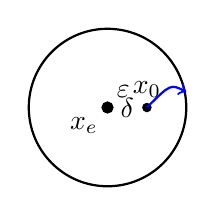
\begin{tikzpicture}[scale=1.0]
        % epsilon circle
        \draw[thick] (0,0) circle (\epsrad);
        \node at (\epsrad+0.2,0.2) {$\varepsilon$};
        % delta circle
        \draw[dashed] (0,0) circle (\deltarad);
        \node at (0.25,0.0) {$\delta$};
        % equilibrium
        \filldraw[black] (0,0) circle (2pt) node[below left] {$x_e$};
        % initial point x0
        \filldraw[black] (0.5,0.0) circle (1.5pt) node[above] {$x_0$};
        % trajectory: stays within epsilon
        \draw[->,blue,thick] (0.5,0.0) .. controls (0.8,0.3) .. (1.0,0.2);
    \end{tikzpicture}
    \caption{Stable: perturbation remains inside $\varepsilon$}
    \end{subfigure}
    \hfill
    %---------------- (b) Convergent ----------------
    \begin{subfigure}[b]{0.45\textwidth}
    \centering
    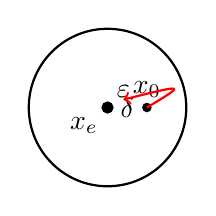
\begin{tikzpicture}[scale=1.0]
        % epsilon circle
        \draw[thick] (0,0) circle (\epsrad);
        \node at (\epsrad+0.2,0.2) {$\varepsilon$};
        % delta circle
        \draw[dashed] (0,0) circle (\deltarad);
        \node at (0.25,0.0) {$\delta$};
        % equilibrium
        \filldraw[black] (0,0) circle (2pt) node[below left] {$x_e$};
        % initial point x0
        \filldraw[black] (0.5,0.0) circle (1.5pt) node[above] {$x_0$};
        % trajectory: moves outward then comes back
        \draw[->,red,thick] (0.5,0.0) .. controls (1.0,0.3) .. (0.2,0.1);
    \end{tikzpicture}
    \caption{Convergent: trajectories return to $x_e$}
    \end{subfigure}
    
    \vspace{0.8cm}
    
    %---------------- (c) Asymptotic stability ----------------
    \begin{subfigure}[b]{0.45\textwidth}
    \centering
    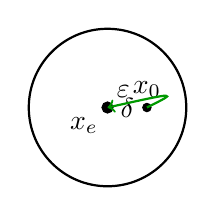
\begin{tikzpicture}[scale=1.0]
        % epsilon circle
        \draw[thick] (0,0) circle (\epsrad);
        \node at (\epsrad+0.2,0.2) {$\varepsilon$};
        % delta circle
        \draw[dashed] (0,0) circle (\deltarad);
        \node at (0.25,0.0) {$\delta$};
        % equilibrium
        \filldraw[black] (0,0) circle (2pt) node[below left] {$x_e$};
        % initial point x0
        \filldraw[black] (0.5,0.0) circle (1.5pt) node[above] {$x_0$};
        % trajectory: goes slightly outward then converges back
        \draw[->,green!60!black,thick] (0.5,0.0) .. controls (0.9,0.2) .. (0.0,0.0);
    \end{tikzpicture}
    \caption{Asymptotically Stable: stable + convergent}
    \end{subfigure}
    \hfill
    %---------------- (d) Exponential stability ----------------
    \begin{subfigure}[b]{0.45\textwidth}
    \centering
    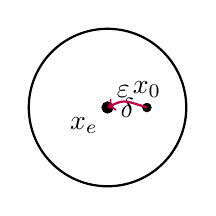
\begin{tikzpicture}[scale=1.0]
        % epsilon circle
        \draw[thick] (0,0) circle (\epsrad);
        \node at (\epsrad+0.2,0.2) {$\varepsilon$};
        % delta circle
        \draw[dashed] (0,0) circle (\deltarad);
        \node at (0.25,0.0) {$\delta$};
        % equilibrium
        \filldraw[black] (0,0) circle (2pt) node[below left] {$x_e$};
        % initial point x0
        \filldraw[black] (0.5,0.0) circle (1.5pt) node[above] {$x_0$};
        % trajectory: sharp fast decay to equilibrium
        \draw[->,purple,thick] (0.5,0.0) .. controls (0.2,0.1) .. (0.0,0.0);
    \end{tikzpicture}
    \caption{Exponentially Stable: fast decay $\sim e^{-\alpha t}$}
    \end{subfigure}

    \caption{Illustrations of stability concepts around equilibrium $x_e$: 
    all trajectories start at an initial condition $x_0$ inside the $\delta$-ball 
    and evolve differently depending on the stability type.}
\end{figure}

%------------------------------------------------
\section{Positive Definite Functions}\index{Positive Definite Functions}

Positive definite functions are the basis of Lyapunov stability theory.  
They provide a way to measure the ``energy'' of a system and are crucial for analyzing stability.

\begin{definition}[Positive Semidefinite Function]
A continuous function $V:\mathcal{D}\subset\mathbb{R}^n \to \mathbb{R}$ is said to be
\begin{itemize}
    \item \textbf{Positive semidefinite} if 
    \[
        V(x) \geq 0, \quad \forall x \in \mathcal{D}, \quad V(0) = 0
    \]
    \item \textbf{Positive definite} if 
    \[
        V(x) > 0 \ \forall x \in \mathcal{D}\setminus\{0\}, \quad V(0)=0
    \]
    \item \textbf{Negative semidefinite} if $V(x) \leq 0$ with equality at the origin.
    \item \textbf{Negative definite} if $V(x) < 0$ for all $x \neq 0$ and $V(0)=0$.
\end{itemize}
\end{definition}

\begin{example}[Quadratic Form]
An important class of functions is given by quadratic forms:
\[
    V(x) = x^T Q x, \quad Q = Q^T \in \mathbb{R}^{n\times n}.
\]
Here,
\begin{itemize}
    \item If $Q$ is positive definite, then $V(x)$ is positive definite.
    \item If $Q$ is positive semidefinite, then $V(x)$ is positive semidefinite.
\end{itemize}
\end{example}

\begin{definition}[Lie Derivative]
Consider a dynamical system 
\[
    \dot{x} = f(x), \quad f:\mathcal{D}\subset\mathbb{R}^n \to \mathbb{R}^n.
\]
For a differentiable function $V:\mathcal{D}\to \mathbb{R}$, the \textbf{Lie derivative} of $V$ along $f$ is defined as
\[
    \dot{V}(x) = L_f V(x) = \nabla V(x)\cdot f(x) =\frac{\partial V}{\partial x}f(x)
\]
\end{definition}

\begin{example}[Computation of $\dot V(x)$]
Consider the nonlinear system
\[
    \dot{x}_1 = 2x_1, 
    \qquad 
    \dot{x}_2 = x_1x_2,
\]
with state vector $x = \begin{bmatrix}x_1 \\ x_2\end{bmatrix}$.

Let the candidate Lyapunov function be
\[
    V(x) = x_1^2 + x_2^2.
\]

Then the gradient of $V$ is
\[
    \nabla V(x) = \begin{bmatrix} 2x_1 & 2x_2 \end{bmatrix}.
\]

Hence the Lie derivative of $V$ along $f(x)$ is
\[
    \dot{V}(x) = \nabla V(x)\cdot f(x) 
    = \begin{bmatrix} 2x_1 & 2x_2 \end{bmatrix}
      \begin{bmatrix} 2x_1 \\ x_1x_2 \end{bmatrix}.
\]

Carrying out the multiplication,
\[
    \dot{V}(x) = 4x_1^2 + 2x_1x_2^2.
\]

\end{example}

\begin{remark}
The sign of $\dot{V}(x)$ (negative definite, semidefinite, or indefinite) determines whether the function $V$ can be used as a Lyapunov function to prove stability of the equilibrium at the origin.
\end{remark}

%------------------------------------------------
\section{Stability Theorems}\index{Stability Theorems}

\begin{theorem}[Lyapunov Stability Theorem]
Consider the autonomous system
\[
    \dot{x} = f(x), \qquad f(0)=0,
\]
with equilibrium at the origin.  
Let $V:\mathcal{D}\to \mathbb{R}$ be a continuously differentiable function such that:
\begin{enumerate}
    \item $V(0) = 0$,
    \item $V(x) > 0, \quad \forall x \in \mathcal{D}\setminus\{0\}$ (positive definite),
    \item $\dot V(x) = \nabla V(x)\cdot f(x) \leq 0, \quad \forall x \in \mathcal{D}\setminus\{0\}$.
\end{enumerate}
Then the equilibrium at the origin is \textbf{stable}.
\end{theorem}

\begin{theorem}[Asymptotic Stability Theorem]
Under the same setup, suppose:
\begin{enumerate}
    \item $V(0) = 0$,
    \item $V(x) > 0, \quad \forall x \in \mathcal{D}\setminus\{0\}$,
    \item $\dot V(x) < 0, \quad \forall x \in \mathcal{D}\setminus\{0\}$ (negative definite).
\end{enumerate}
Then the equilibrium at the origin is \textbf{asymptotically stable}.
\end{theorem}

\begin{example}[Pendulum without Friction]
Consider the undamped pendulum (schematic shown below):

\begin{center}
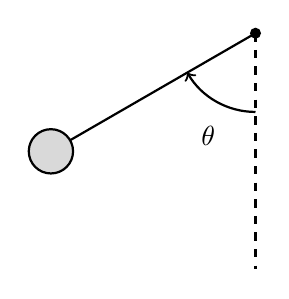
\begin{tikzpicture}[thick,scale=1.0]
    % Pivot point
    \fill (0,0) circle (2pt);

    % String
    \draw (0,0) -- (30:-3);

    % Bob
    \filldraw[fill=gray!30] (30:-3) circle (8pt);

    % Vertical reference line
    \draw[dashed] (0,0) -- (0,-3);

    % Angle theta
    \draw[->] (0,-1) arc (-90:-150:1);
    \node at (-0.6,-1.3) {$\theta$};
\end{tikzpicture}
\end{center}

The dynamics are:
\[
    \ddot{\theta} + \frac{g}{l}\sin\theta = 0.
\]
Define the state variables $x_1 = \theta$, $x_2 = \dot\theta$.  
The system can be written as:
\[
    \dot{x}_1 = x_2, 
    \qquad 
    \dot{x}_2 = -\tfrac{g}{l}\sin(x_1).
\]

Choose the candidate Lyapunov function (total mechanical energy):
\[
    V(x) = \tfrac{1}{2}x_2^2 + \tfrac{g}{l}(1-\cos x_1).
\]

Then
\[
    \dot V(x) = \nabla V(x)\cdot f(x) = x_2\dot{x}_2 + \tfrac{g}{l}\sin(x_1)\dot{x}_1 = 0.
\]

Hence $\dot V(x)=0$, so $V$ is conserved (energy conservation).  
The equilibrium is \textbf{stable}, but not asymptotically stable.
\end{example}


\begin{example}[Pendulum with Friction]
Now consider the damped pendulum:
\[
    \ddot{\theta} + k\dot{\theta} + \tfrac{g}{l}\sin\theta = 0, \quad k>0.
\]
In state-space form:
\[
    \dot{x}_1 = x_2, 
    \qquad 
    \dot{x}_2 = -k x_2 - \tfrac{g}{l}\sin(x_1).
\]

Using the same Lyapunov function:
\[
    V(x) = \tfrac{1}{2}x_2^2 + \tfrac{g}{l}(1-\cos x_1),
\]
we compute
\[
    \dot V(x) = x_2\dot{x}_2 + \tfrac{g}{l}\sin(x_1)\dot{x}_1
    = x_2(-k x_2 - \tfrac{g}{l}\sin(x_1)) + \tfrac{g}{l}\sin(x_1)x_2.
\]

Simplifying,
\[
    \dot V(x) = -k x_2^2 \leq 0,
\]
with equality only when $x_2=0$.  

Thus, $\dot V(x)<0$ for all $x_2 \neq 0$, and the equilibrium is \textbf{asymptotically stable}.
\end{example}

\newpage
%------------------------------------------------
\section{Asymptotic Stability in the Large}\index{Asymptotic Stability in the Large}

\begin{definition}[Global Asymptotic Stability]
	An equilibrium point $x_e$ of $\dot{x}=f(x)$ is said to be \emph{globally asymptotically stable} if it is:
	\begin{enumerate}
		\item Stable in the sense of Lyapunov;
		\item For every initial condition $x(0)\in \mathbb{R}^n$, $\lim_{t\to\infty}x(t)=x_e$.
	\end{enumerate}
\end{definition}

\begin{definition}[Radially Unbounded Function]
	A continuously differentiable function $V:\mathbb{R}^n \to \mathbb{R}$ is said to be \emph{radially unbounded} if
	\begin{equation}
		\|x\| \to \infty \quad \Rightarrow \quad V(x)\to \infty.
	\end{equation}
	In other words, the value of $V(x)$ increases without bound as the norm of $x$ goes to infinity.
\end{definition}

\begin{theorem}[Lyapunov’s Global Stability Theorem]
	Consider the system $\dot{x}=f(x)$ with equilibrium at $x=0$.  
	If there exists a continuously differentiable function $V:\mathbb{R}^n \to \mathbb{R}$ such that:
	\begin{enumerate}
		\item $V(0)=0$,
		\item $V(x)>0$ for all $x\neq 0$,
		\item $V(x)\to \infty$ as $\|x\|\to \infty$ (radially unbounded),
		\item $\dot{V}(x)<0$ for all $x\neq 0$,
	\end{enumerate}
	then the equilibrium $x=0$ is globally asymptotically stable.
\end{theorem}

\begin{example}[Mass–Spring–Damper]
	Consider a mass--spring--damper system:
	\begin{equation}
		m\ddot{x} + c\dot{x} + kx = 0, \quad m,c,k>0.
	\end{equation}
	Choose the Lyapunov function representing the total energy:
	\begin{equation}
		V(x,\dot{x}) = \tfrac{1}{2}m\dot{x}^2 + \tfrac{1}{2}kx^2.
	\end{equation}
	Then:
	\begin{itemize}
		\item $V(x,\dot{x}) \ge 0$, and $V(x,\dot{x}) \to \infty$ as $\|(x,\dot{x})\|\to \infty$ (radially unbounded),
		\item $\dot{V}(x,\dot{x}) = -c\dot{x}^2 < 0$ for $\dot{x}\neq 0$.
	\end{itemize}
	Thus, the equilibrium point $(x,\dot{x})=(0,0)$ is globally asymptotically stable:  
	the mass always comes to rest at the origin, regardless of its initial displacement and velocity.
\end{example}


%------------------------------------------------
\section{Positive Definite Functions Revisited}\index{Positive Definite Functions Revisited}

\begin{definition}[Class $\mathcal{K}$ Functions]
	A continuous function $\alpha:[0,a)\to [0,\infty)$ is said to belong to \emph{class $\mathcal{K}$} if it is:
	\begin{enumerate}
		\item strictly increasing,
		\item $\alpha(0)=0$.
	\end{enumerate}
	If $a=\infty$ and $\alpha(r)\to \infty$ as $r\to \infty$, then $\alpha$ is said to be of \emph{class $\mathcal{K}_\infty$}.
\end{definition}

\begin{corollary}
	A function $V:\mathbb{R}^n \to \mathbb{R}$ is positive definite if and only if there exist class $\mathcal{K}$ functions $\alpha_1, \alpha_2$ such that
	\begin{equation}
		\alpha_1(\|x\|) \leq V(x) \leq \alpha_2(\|x\|), \quad \forall x \in \mathbb{R}^n.
	\end{equation}
\end{corollary}

\begin{corollary}
	Let $x_e$ be an equilibrium of $\dot{x}=f(x)$.  
	If there exists a continuous positive definite function $V(x)$ such that $\dot{V}(x) \leq 0$, then $x_e$ is stable.
\end{corollary}

\begin{corollary}
	Let $x_e$ be an equilibrium of $\dot{x}=f(x)$.  
	If there exists a continuous positive definite function $V(x)$ such that $\dot{V}(x) < 0$ for all $x\neq x_e$, then $x_e$ is asymptotically stable.
\end{corollary}

%------------------------------------------------
\subsection{Exponential Stability}\index{Positive Definite Functions Revisited!Exponential Stability}

\begin{theorem}[Exponential Stability]
	Consider the system $\dot{x}=f(x)$ with equilibrium at $x=0$.  
	If there exists a continuously differentiable, radially unbounded, positive definite function $V(x)$ such that
	\begin{equation}
		c_1 \|x\|^2 \leq V(x) \leq c_2 \|x\|^2,
	\end{equation}
	and
	\begin{equation}
		\dot{V}(x) \leq -c_3 \|x\|^2,
	\end{equation}
	for positive constants $c_1, c_2, c_3 > 0$, then the equilibrium $x=0$ is \emph{globally exponentially stable}.  
	In particular, there exist constants $k,\lambda > 0$ such that
	\begin{equation}
		\|x(t)\| \leq k e^{-\lambda t}\|x(0)\|, \quad \forall t \geq 0.
	\end{equation}
\end{theorem}

\begin{example}[Linear system: global exponential stability]
Consider the system
\begin{equation}
    \dot{x} = Ax,\qquad A=\begin{bmatrix}-1 & 0\\ 0 & -2\end{bmatrix}.
\end{equation}
Choose the Lyapunov function $V(x)=\tfrac{1}{2}\|x\|^2=\tfrac{1}{2}(x_1^2+x_2^2)$. Then
\begin{equation}
    \dot{V}(x) = x^\top \dot{x} = x_1(-x_1)+x_2(-2x_2) = -x_1^2-2x_2^2
    \le -\min\{1,2\}\,(x_1^2+x_2^2) = -\|x\|^2.
\end{equation}
Moreover,
\begin{equation}
    \tfrac{1}{2}\|x\|^2 \le V(x) \le \tfrac{1}{2}\|x\|^2, 
    \qquad \dot{V}(x) \le -\|x\|^2 = -2\,V(x).
\end{equation}
By the exponential stability theorem, $x=0$ is \emph{globally exponentially stable} and
\begin{equation}
    \|x(t)\| \le e^{-t}\|x(0)\|.
\end{equation}
\end{example}

\begin{example}[Nonlinear system: global exponential stability]
Consider the scalar system
\begin{equation}
    \dot{x} = -x - x^3.
\end{equation}
Let $V(x)=\tfrac{1}{2}x^2$. Then
\begin{equation}
    \dot{V}(x) = x\dot{x} = x(-x-x^3) = -x^2 - x^4 \le -x^2 = -2V(x).
\end{equation}
Hence $V$ is positive definite and satisfies $\dot{V}\le -2V$ globally, so the origin is
\emph{globally exponentially stable}. In particular,
\begin{equation}
    |x(t)| \le e^{-t}\,|x(0)|.
\end{equation}
\end{example}

\begin{remark}[Contrast: asymptotic but not exponential]
For the system $\dot{x}=-x^3$ with $V(x)=\tfrac{1}{2}x^2$, we get $\dot{V}=-x^4$.
Although $\dot{V}<0$ for $x\neq 0$ (implying global asymptotic stability), there is no bound of the form
$\dot{V}\le -c\,V$ with a constant $c>0$ valid for all $x$. Thus the origin is \emph{not} exponentially
stable—only (global) asymptotically stable.
\end{remark}

\section{Construction of Lyapunov Functions}\index{Construction of Lyapunov Functions}

We present the \emph{variable-gradient} (also called ``line-integral'') method for constructing a scalar Lyapunov function \(V(x)\) from a candidate gradient field \(g(x)\). The main theorem gives a simple necessary and sufficient condition when a vector field is a gradient.

\begin{theorem}
Let \(G\subset\mathbb{R}^n\) be open and simply connected. A continuously differentiable vector field \(g:G\to\mathbb{R}^n\) is the gradient of a scalar function \(V:G\to\mathbb{R}\) (that is, \(g=\nabla V\)) if and only if the Jacobian matrix \(Dg(x)\) is symmetric for all \(x\in G\):
\[
\frac{\partial g_i}{\partial x_j}(x)=\frac{\partial g_j}{\partial x_i}(x)
\quad\text{for all }i,j,\ x\in G.
\]
\end{theorem}

\subsection{Variable-gradient method}\index{Construction of Lyapunov Functions!Variable-gradient method}
Given a candidate vector field \(g(x)\) (continuous and \(C^1\)) on a simply connected domain:

\begin{enumerate}
  \item \textbf{Check symmetry:} compute the Jacobian \(Dg(x)\). Verify \(\partial g_i/\partial x_j=\partial g_j/\partial x_i\) for all \(i,j\). If not symmetric, \(g\) is not a gradient and the method fails.
  \item \textbf{Construct \(V\):} if symmetric, define
  \[
  V(x)=\int_{0}^{1} x^\top g(tx)\,dt
  \]
  or pick a base point \(x_0\) and set
  \[
  V(x)=\int_{\gamma} g(\xi)\cdot d\xi,
  \]
  where \(\gamma\) is any path from \(x_0\) to \(x\). Path independence holds because \(Dg\) is symmetric.
  \item \textbf{Verify gradient:} differentiate the built \(V\) to confirm \(\nabla V(x)=g(x)\).
  \item \textbf{Lyapunov test (for dynamics):} for a system \(\dot x=f(x)\), if you choose \(f(x)=-g(x)\) then
  \[
  \dot V(x)=\nabla V(x)\cdot\dot x = g(x)\cdot(-g(x))=-\|g(x)\|^2\le 0,
  \]
  so \(V\) is a (nonincreasing) Lyapunov function; it is positive definite if \(V(0)=0\) and \(V(x)>0\) for \(x\neq0\).
\end{enumerate}

\begin{example}
Consider the nonlinear system
\[
\dot{x}_1=-a x_1,\qquad \dot{x}_2= b x_2 + x_1x_2^2,\qquad a>0.
\]

\begin{enumerate}
\item \textbf{Choose candidate gradient field.}  
\\Take
$
g(x)=\begin{bmatrix}2x_1\\ x_2\end{bmatrix}.
$
Its Jacobian is
$
Dg(x)=\begin{bmatrix}2 & 0\\0 & 1\end{bmatrix},
$
which is symmetric.

\item \textbf{Construct \(V(x)\).}  
Integrating gives
\[
V(x)=x_1^2+\tfrac{1}{2}x_2^2,
\]
since \(\nabla V(x)=g(x)\).

\item \textbf{Verify Lyapunov conditions.}  
\\Clearly, \(V(x)>0\) for all \(x\neq 0\) and \(V(0)=0\). Along trajectories,
\[
\dot{V}(x)=\nabla V(x)\cdot \dot{x}
=\begin{bmatrix}2x_1 & x_2\end{bmatrix}
\begin{bmatrix}-a x_1\\ b x_2+x_1x_2^2\end{bmatrix}.
\]

Carrying out the multiplication,
\[
\dot{V}(x)=-2a x_1^2+b x_2^2+x_1x_2^3.
\]

\item \textbf{Interpretation.}  
\\- If \(b<0\) and the cross-term \(x_1x_2^3\) is small (e.g., in a local region around the origin), then \(\dot{V}(x)\leq 0\).  
\\- Thus, \(V(x)\) serves as a Lyapunov function showing local stability of the origin when \(a>0,\ b<0\).
\end{enumerate}
\end{example}

\begin{remark}
\textbf{How do we choose $g(x)$ in the variable-gradient method?}

\begin{itemize}
  \item Start with a quadratic candidate $V(x)=p_1x_1^2+p_2x_2^2+\cdots$, with $p_i>0$.  
        Its gradient is $g(x)=[2p_1x_1,\ 2p_2x_2,\ \ldots]^T$.  

  \item Check $\dot V(x)=g(x)^\top f(x)$.  
        Adjust the constants $p_i$ so that the negative terms dominate.  

  \item For the system 
  \[
  \dot{x}_1=-a x_1,\qquad \dot{x}_2=b x_2+x_1x_2^2,
  \]
  the simple choice $g(x)=[2x_1,\ x_2]^T$ works well, leading to
  $V(x)=x_1^2+\tfrac12 x_2^2$.

  \item In general, if cross-terms appear in $\dot V(x)$, try adding cross-terms
  like $x_1x_2$ inside $V(x)$ so that $g(x)$ cancels unwanted terms.
\end{itemize}
\end{remark}

\section{The Invariance Principle}\index{The Invariance Principle}

\begin{definition}[Invariant set]
A set $M \subset \mathbb{R}^n$ is said to be \emph{invariant} with respect to a dynamical system 
\[
\dot{x}=f(x), \quad x(0)=x_0,
\]
if every trajectory starting in $M$ remains in $M$ for all future time, i.e.
\[
x(0)\in M \;\;\Rightarrow\;\; x(t)\in M \quad \forall t\geq 0.
\]
\end{definition}

%--------------------------------------

\begin{theorem}[Asymptotic stability of the origin]
Consider the system $\dot{x}=f(x)$ with equilibrium $x=0$.  
If there exists a continuously differentiable function $V:\mathbb{R}^n\to \mathbb{R}$ such that
\[
V(x)>0 \;\; \forall x\neq 0, \quad V(0)=0, \quad \dot V(x) = \nabla V(x)\cdot f(x) <0 \;\; \forall x\neq 0,
\]
then the equilibrium $x=0$ is \emph{asymptotically stable}.
\end{theorem}

\begin{example}
For $\dot{x}=-x$ in $\mathbb{R}$, choose $V(x)=\tfrac12 x^2$. Then $V(x)>0$ for $x\neq 0$, and
\[
\dot V(x) = x(-x) = -x^2 <0.
\]
Hence $x=0$ is asymptotically stable.
\end{example}

%--------------------------------------

\begin{theorem}[Null solution stability for autonomous systems]
Let $\dot{x}=f(x)$ be an autonomous system with equilibrium $x=0$.  
If there exists $V(x)$ positive definite such that $\dot V(x)$ is negative definite, then the \emph{null solution} $x(t)\equiv 0$ is asymptotically stable.
\end{theorem}

\begin{example}
Consider $\dot{x}_1=-x_1+x_2^2,\ \dot{x}_2=-2x_2$.  
Take $V(x)=x_1^2+x_2^2$. Then
\[
\dot V=2x_1(-x_1+x_2^2)+2x_2(-2x_2)=-2x_1^2+2x_1x_2^2-4x_2^2.
\]
For small $x$, negative terms dominate, showing asymptotic stability of the null solution.
\end{example}

%--------------------------------------

\begin{theorem}[LaSalle's Invariance Principle]
Let $\dot{x}=f(x)$ be an autonomous system with equilibrium $x=0$.  
Suppose there exists $V(x)\geq 0$, continuously differentiable, such that $\dot V(x)\leq 0$ in a domain $D$ containing the origin.  
Let 
\[
E=\{x\in D:\dot V(x)=0\}.
\]
If the largest invariant set $M\subset E$ contains only the point $x=0$, then the origin is asymptotically stable.
\end{theorem}

\begin{example}
Consider
\[
\dot{x}_1=-x_1,\qquad \dot{x}_2=-x_1^2.
\]
Take $V(x)=\tfrac12 x_1^2+\tfrac12 x_2^2$. Then
\[
\dot V= x_1(-x_1)+x_2(-x_1^2)=-x_1^2 -x_1^2x_2 \leq 0.
\]
The set where $\dot V=0$ is $\{(0,x_2):x_2\in\mathbb{R}\}$.  
On this set, the dynamics reduce to $\dot{x}_1=0,\ \dot{x}_2=0$, so the only invariant point is $(0,0)$.  
By LaSalle’s theorem, $(0,0)$ is asymptotically stable.
\end{example}

\section{Region of Attraction}\index{Region of Attraction}

\begin{definition}[Trajectory and Region of Attraction]
Let $\psi(x,t)$ denote the trajectory of the system
\[
\dot{x}=f(x), \qquad x(0)=x,
\]
at time $t\geq 0$.  
The \emph{region of attraction} ($R_A$) of an equilibrium point $x_e$ with domain $D\subset \mathbb{R}^n$ is defined as
\[
R_A(x_e)=\{x\in D:\lim_{t\to\infty}\psi(x,t)=x_e\}.
\]
\end{definition}

%--------------------------------------

\begin{theorem}[Lyapunov characterization of region of attraction]
Let $x_e$ be an equilibrium of $\dot{x}=f(x)$ with domain $D$.  
Assume:
\begin{enumerate}
    \item $M\subset D$ is a compact set containing $x_e$ in its interior.
    \item There exists a continuously differentiable function $V:M\to\mathbb{R}$ such that
    \[
    V(x)>0 \ \ \forall x\in M,\ x\neq x_e,\quad V(x_e)=0,
    \]
    and
    \[
    \dot V(x)=\nabla V(x)\cdot f(x) < 0 \quad \forall x\in M,\ x\neq x_e, \qquad \dot V(x_e)=0.
    \]
\end{enumerate}
Then $M\subset R_A(x_e)$, i.e. $M$ is contained in the region of attraction of $x_e$.
\end{theorem}

%--------------------------------------

\begin{example}
Consider the nonlinear system
\[
\dot{x}_1=-x_1+x_1x_2, 
\qquad 
\dot{x}_2=-x_2.
\]
The equilibrium is $x_e=(0,0)$.

Choose the Lyapunov function
\[
V(x)=x_1^2+x_2^2.
\]
Then
\[
\dot V=2x_1(-x_1+x_1x_2)+2x_2(-x_2)=-2x_1^2+2x_1^2x_2-2x_2^2.
\]
\\
\textbf{Analysis:}  \\
- Inside the compact set $M=\{x\in\mathbb{R}^2: V(x)\leq 1\}$, $V$ is positive definite.  
\\- For small $x_2$, the term $2x_1^2x_2$ is dominated by $-2x_1^2-2x_2^2$, hence $\dot V<0$ for all $x\in M$, $x\neq 0$.  
\\- Thus, by the theorem, $M\subset R_A(0)$.
\\So the unit ball $M$ lies inside the region of attraction of the origin.
\end{example}

\section{Analysis of LTI systems}\index{Analysis of LTI systems}

Consider the linear time-invariant (LTI) system
\[
\dot x = A x,\qquad x\in\mathbb{R}^n.
\]

We propose a quadratic Lyapunov candidate
\[
V(x)=x^\top P x, \quad P=P^\top>0.
\]

Differentiating along trajectories gives
\[
\dot V(x) = \dot x^\top P x + x^\top P \dot x 
          = (A x)^\top P x + x^\top P (A x).
\]

This simplifies to
\[
\dot V(x) = x^\top \big(A^\top P + P A\big) x.
\]

To ensure stability, we require \(\dot V(x)<0\) for all \(x\neq 0\).  
A standard way is to enforce
\[
A^\top P + P A = -Q,
\]
where \(Q=Q^\top>0\).  
Thus, \(\dot V(x) = -x^\top Q x < 0\), proving that \(V(x)\) is strictly decreasing along trajectories.

\begin{theorem}[Stability of LTI systems]
Let \(A\in\mathbb{R}^{n\times n}\).
\begin{enumerate}
  \item If all eigenvalues of \(A\) satisfy \(\Re(\lambda)<0\) (i.e. \(A\) is Hurwitz), then the equilibrium \(x=0\) is \textbf{asymptotically stable}.
  \item Equivalently, for any symmetric \(Q=Q^\top>0\), there exists a unique \(P=P^\top>0\) that solves the Lyapunov equation
  \[
  A^\top P + P A = -Q.
  \]
  In this case, the Lyapunov function \(V(x)=x^\top P x\) satisfies
  \[
  \dot V(x) = -x^\top Q x < 0 \quad (x\neq 0).
  \]
\end{enumerate}
\end{theorem}

\begin{remark}
The matrix \(Q\) appears from the requirement that \(\dot V(x)\) must be negative definite.  
It is chosen arbitrarily as any symmetric positive definite matrix, and then \(P\) is solved from the Lyapunov equation.  
Different choices of \(Q\) yield different \(P\), but all provide valid Lyapunov functions proving stability.
\end{remark}

\begin{example}
Take
\[
A=\begin{bmatrix}-1 & 0\\[4pt] 0 & -2\end{bmatrix}, \qquad 
Q=\begin{bmatrix}1 & 0\\[4pt] 0 & 1\end{bmatrix}.
\]
The Lyapunov equation
\[
A^\top P + P A = -Q
\]
becomes
\[
\begin{bmatrix}-1 & 0\\[4pt] 0 & -2\end{bmatrix}
P + P
\begin{bmatrix}-1 & 0\\[4pt] 0 & -2\end{bmatrix}
= -I.
\]

Solving gives
\[
P=\begin{bmatrix}\tfrac12 & 0\\[4pt] 0 & \tfrac14\end{bmatrix}>0.
\]

Thus,
\[
V(x)=\tfrac12 x_1^2+\tfrac14 x_2^2, \qquad 
\dot V(x) = -x_1^2 - x_2^2 < 0 \quad (x\neq 0).
\]

Therefore, the equilibrium \(x=0\) is exponentially asymptotically stable.
\end{example}

\section{Instability}\index{Instability}

\begin{theorem}[Chetaev's Theorem]
Consider the system $\dot x = f(x)$ with equilibrium at $x=0$.  
If there exists a continuously differentiable function $V(x)$ such that:
\begin{enumerate}
  \item $V(0)=0$,
  \item $V(x)>0$ in some neighborhood of the origin (except at $x=0$),
  \item $\dot V(x)>0$ in that neighborhood,
\end{enumerate}
then the equilibrium $x=0$ is \textbf{unstable}.
\end{theorem}

\begin{remark}
This result is the dual of Lyapunov’s stability theorem:  
instead of $\dot V(x)<0$ implying stability, here $\dot V(x)>0$ implies instability.
\end{remark}

\begin{example}
Consider the scalar system
\[
\dot x = x.
\]
Choose
\[
V(x) = \tfrac{1}{2} x^2.
\]
We check Chetaev’s conditions:
\begin{align*}
V(0) &= 0, \\
V(x) &= \tfrac{1}{2}x^2 > 0 \quad \text{for } x\neq 0, \\
\dot V(x) &= x \dot x = x(x) = x^2 > 0 \quad \text{for } x\neq 0.
\end{align*}
Thus, all conditions are satisfied, and by Chetaev’s theorem,  
the equilibrium $x=0$ is unstable.
\end{example}

\chapterimage{orange2.jpg} % Chapter heading image
\chapterspaceabove{6.75cm} % Whitespace from the top of the page to the chapter title on chapter pages
\chapterspacebelow{7.25cm} % Amount of vertical whitespace from the top margin to the start of the text on chapter pages

\chapter{Lyapunov Stability II: Nonautonomous Systems}\index{Lyapunov Stability II: Nonautonomous Systems}

\section{Overview}\index{Overview}
In the previous chapter, we studied autonomous systems, where the dynamics depend only on the state variables. We now extend the discussion to \textbf{nonautonomous systems}, where time explicitly appears as a second variable in the system dynamics. Such systems are represented as
\[
\dot{x}(t) = f(x,t), \quad x \in \mathbb{R}^n, \; t \in \mathbb{R}.
\]

The presence of time makes the analysis more challenging, since the system’s behavior may vary depending on when an input or disturbance is applied. For example, equilibrium points can shift or even cease to exist in the classical sense, and stability must be understood relative to a time-varying reference.

In this chapter, we adapt Lyapunov’s direct method to nonautonomous systems by introducing \textbf{Lyapunov functions with explicit time dependence} \( V(x,t) \). This allows us to study stability notions such as \textit{uniform stability}, \textit{uniform asymptotic stability}, and \textit{exponential stability}, which are crucial in time-varying and control-driven systems.

This framework broadens the applicability of Lyapunov’s theory, enabling the analysis of systems with time-varying parameters, switching dynamics, and external inputs---common in modern control applications.

%------------------------------------------------
\section{Definitions}\index{Definitions}

\begin{definition}[Stability Concepts]
Consider the system $\dot{x}=f(x,t)$ with equilibrium $x=0$.  
\begin{itemize}
    \item \textbf{Stable:} For every $\epsilon>0$ and $t_0$, there exists $\delta(\epsilon,t_0)>0$ such that
    \[
    ||x(t_0)|| < \delta \;\; \Rightarrow \;\; ||x(t)|| < \epsilon, \quad \forall t \geq t_0.
    \]
    \item \textbf{Convergent:} $x(t) \to 0$ as $t \to \infty$.
    \item \textbf{Asymptotically Stable:} The equilibrium is stable and convergent.  
    \item \textbf{Unstable:} The equilibrium is not stable.  
\end{itemize}
\end{definition}

\begin{definition}[Uniform Stability Concepts]
The equilibrium $x=0$ is said to be uniformly stable if the $\delta$ in the stability definition is independent of $t_0$.  
\begin{itemize}
    \item \textbf{Uniformly Stable:} $\delta = \delta(\epsilon)$ independent of $t_0$.  
    \item \textbf{Uniformly Convergent:} For every $\epsilon>0$, there exists $T(\epsilon)>0$ independent of $t_0$ such that
    \[
    t \geq t_0 + T(\epsilon) \;\; \Rightarrow \;\; ||x(t)|| < \epsilon.
    \]
    \item \textbf{Uniformly Asymptotically Stable (UAS):} Uniformly stable and uniformly convergent.  
    \item \textbf{Globally Uniformly Asymptotically Stable (GUAS):} Uniformly asymptotically stable with region of attraction $\mathbb{R}^n$.  
\end{itemize}
\end{definition}

\begin{definition}[Exponential Stability]
The equilibrium $x=0$ is \textbf{exponentially stable} if there exist constants $\alpha>0$, $\lambda>0$, and $\delta>0$ such that
\[
||x(t)|| \leq \alpha \, ||x(t_0)|| e^{-\lambda (t-t_0)}, \quad \forall t \geq t_0, \; ||x(t_0)|| < \delta.
\]
If the inequality holds for all $x(t_0)\in\mathbb{R}^n$, the equilibrium is \textbf{globally exponentially stable}.
\end{definition}

%------------------------------------------------
\section{Positive Definite Functions}\index{Positive Definite Functions}

Let $W : D \times \mathbb{R}^+ \to \mathbb{R}$ be a scalar function, where $D \subseteq \mathbb{R}^n$ is a domain containing the origin.  
Assume that $W(x,t)$ is continuous in $(x,t)$ and has continuous partial derivatives with respect to $x$.

\begin{definition}[Positive Semi-Definite Function]
A function $W(x,t)$ is said to be \textbf{positive semi-definite} in $D$ if
\[
W(0,t) = 0 \forall t \in \mathbb{R}^+
\]
\[
W(x,t) \geq 0, \quad \forall (x,t) \in D \times \mathbb{R}^+.
\]
\end{definition}

\begin{definition}[Positive Definite Function]
A function $W(x,t)$ is said to be \textbf{positive definite} in $D$ if
\[
W(0,t) = 0, \quad W(x,t) > 0 \;\; \forall x \neq 0,
\]
and there exists a continuous function $V_1(x)$ with $V_1(0)=0$ such that
\[
V_1(x) \leq W(x,t), \quad \forall (x,t) \in D \times \mathbb{R}^+.
\]
\end{definition}

\begin{definition}[Decrescent Function]
A function $W(x,t)$ is said to be \textbf{decrescent} in $D$ if there exists a continuous function $V_2(x)$ with $V_2(0)=0$ such that
\[
W(x,t) \leq V_2(x), \quad \forall (x,t) \in D \times \mathbb{R}^+.
\]
\end{definition}

\begin{definition}[Radially Unbounded Function]
A function $W(x,t)$ is said to be \textbf{radially unbounded} if
\[
||x|| \to \infty \;\; \Rightarrow \;\; W(x,t) \to \infty, \quad \forall t \geq 0.
\]
\end{definition}

\begin{example}[A single example covering the definitions]
Consider
\[
W(x,t) = \big(1+|\sin t|\big)\,\|x\|^2, 
\qquad x\in\mathbb{R}^n,\; t\ge 0.
\]

\begin{itemize}
    \item \textbf{Regularity:}  
    $W(x,t)$ is continuous in $(x,t)$ and has continuous partial derivatives with respect to $x$.  

    \item \textbf{Positive semi-definite:}  
    Since $\|x\|^2 \ge 0$ and $1+|\sin t|\ge 0$, we have $W(x,t)\ge 0$.  

    \item \textbf{Positive definite:}  
    Because $1+|\sin t|\in [1,2]$,  
    \[
    \|x\|^2 \le W(x,t) \le 2\|x\|^2.
    \]  
    Thus, $W(0,t)=0$ and $W(x,t)>0$ for all $x\neq 0$. One may take $V_1(x)=\|x\|^2$ so that $V_1(x)\le W(x,t)$.

    \item \textbf{Decrescent:}  
    Since $W(x,t)\le 2\|x\|^2$ for all $t$, we can take $V_2(x)=2\|x\|^2$ such that $W(x,t)\le V_2(x)$.  

    \item \textbf{Radially unbounded:}  
    As $\|x\|\to\infty$, we have $W(x,t)\ge \|x\|^2 \to\infty$. Hence $W$ is radially unbounded.  
\end{itemize}

\end{example}

\section{Stability Theorems}\index{Stability Theorems}

\begin{theorem}[Lyapunov Stability Theorem]
Let $W:D\times[0,\infty)\to\mathbb{R}$ be a continuously differentiable function.  
If 
\begin{itemize}
    \item $W(x,t)$ is positive definite in $D$, and  
    \item its derivative along any solution satisfies $\dot{W}(x,t)\le 0$,  
\end{itemize}
then the equilibrium $x=0$ is \textbf{stable}.
\end{theorem}

\begin{theorem}[Lyapunov Uniform Asymptotic Stability]
Suppose there exists $W:D\times[0,\infty)\to\mathbb{R}$ such that
\begin{itemize}
    \item $W(x,t)$ is positive definite and decrescent,  
    \item $\dot{W}(x,t)$ is negative definite,  
\end{itemize}
then the equilibrium $x=0$ is \textbf{uniformly asymptotically stable}.
\end{theorem}

\begin{theorem}[Restated Lyapunov Uniform Asymptotic Stability]
If there exist class-$\mathcal{K}$ functions $v_1, v_2, v_3$ such that
\[
v_1(\|x\|) \;\le\; W(x,t) \;\le\; v_2(\|x\|), 
\]
and
\[
\frac{\partial W}{\partial t}(x,t) + \nabla W(x,t) f(x,t) \;\le\; -v_3(\|x\|),
\]
then the equilibrium $x=0$ is \textbf{uniformly asymptotically stable}.
\end{theorem}

\begin{theorem}[Global Uniform Asymptotic Stability]
Suppose there exists $W:\mathbb{R}^n\times[0,\infty)\to\mathbb{R}$ such that
\begin{itemize}
    \item $W(x,t)$ is positive definite, decrescent, and radially unbounded,  
    \item $\dot{W}(x,t)$ is negative definite,  
\end{itemize}
then the equilibrium $x=0$ is \textbf{globally uniformly asymptotically stable}.
\end{theorem}

\begin{remark}\textbf{Hierarchy of Stability Notions}
\\\\The following chain of implications holds:
\[
\text{Global Uniform Asymptotic Stability} 
\;\;\Rightarrow\;\; \text{Uniform Asymptotic Stability} 
\;\;\Rightarrow\;\; \text{Asymptotic Stability} 
\;\;\Rightarrow\;\; \text{Stability}.
\]
The converse implications do not hold in general.
\end{remark}

\section{Analysis of LTV Systems}\index{Analysis of LTV Systems}

Consider the linear time-varying system
\[
\dot{x}(t) = A(t)x(t), \qquad x(t_0)=x_0,
\]
where $A(t)$ is a continuous matrix function of time.

Let $\Phi(t,t_0)$ denote the \textbf{state transition matrix}, which satisfies
\[
\dot{\Phi}(t,t_0) = A(t)\Phi(t,t_0), 
\qquad \Phi(t_0,t_0) = I.
\]

\begin{theorem}[Exponential Stability via State Transition Matrix]
The equilibrium $x=0$ of the LTV system is \textbf{exponentially stable} if there exist constants $\alpha>0$ and $\lambda>0$ such that
\[
\|\Phi(t,t_0)\| \le \alpha e^{-\lambda (t-t_0)}, 
\qquad \forall t\ge t_0\ge 0.
\]
\end{theorem}

Now consider the quadratic Lyapunov function candidate
\[
W(x,t) = x^T P(t) x,
\]
where $P(t)=P^T(t)>0$ for all $t\ge 0$.  
The derivative along solutions is
\[
\dot{W}(x,t) = x^T \big( \dot{P}(t) + A^T(t)P(t) + P(t)A(t) \big) x.
\]

\begin{theorem}[Exponential Stability via Lyapunov Function]
Suppose there exist positive definite matrices $P(t)$ and $Q(t)$ such that
\[
\dot{P}(t) + A^T(t)P(t) + P(t)A(t) = -Q(t),
\]
with $Q(t)>0$ for all $t\ge 0$.  
Then the equilibrium $x=0$ is \textbf{uniformly exponentially stable}.
\end{theorem}

\begin{remark}\textbf{Origin of $Q(t)$ and Construction of $P(t)$}
\\\\The matrix $Q(t)$ appears as the negative of the quadratic form that equals the derivative of the candidate Lyapunov function:
\[
\dot W(x,t) = x^T\big(\dot P(t)+A^T(t)P(t)+P(t)A(t)\big)x = -x^T Q(t)x.
\]
Thus $Q(t)>0$ guarantees $\dot W \le -\lambda_{\min}(Q(t))\|x\|^2$, which ensures dissipation.

A standard way to obtain a symmetric positive definite $P(t)$ for a given positive definite $Q(t)$ is via the state transition matrix:
\[
P(t) = \int_{t}^{\infty} \Phi^T(\tau,t)\,Q(\tau)\,\Phi(\tau,t)\,d\tau.
\]
If the system is exponentially stable, this integral converges and yields $P(t)$ satisfying the Lyapunov differential equation.

Moreover, if there exist constants $m_1,m_2>0$ such that
\[
m_1 I \le Q(t) \le m_2 I, 
\qquad \alpha_1 I \le P(t) \le \alpha_2 I,
\]
then
\[
\dot W \le -m_1 \|x\|^2 \le -\tfrac{m_1}{\alpha_2}W,
\]
which implies the exponential decay estimate
\[
\|x(t)\| \le \sqrt{\tfrac{\alpha_2}{\alpha_1}} \, e^{-\tfrac{m_1}{2\alpha_2}(t-t_0)} \|x(t_0)\|.
\]
This shows how the choice of $Q(t)$ (and the resulting $P(t)$) provides explicit exponential stability bounds.
\end{remark}

\begin{example}
Consider the time-varying linear system
\[
\dot x(t)=A(t)x(t),\qquad A(t) = -\big(1+\tfrac{1}{2}\sin t\big) I_{2},
\]
so that \(x\in\mathbb{R}^2\) and \(A(t)\) is a scalar multiple of the identity. Note that
\[
a(t):=1+\tfrac{1}{2}\sin t \in [\,1/2,\,3/2\,].
\]

\begin{itemize}
    \item \textbf{State-transition matrix.} Because \(A(t)\) is a scalar times \(I\), the state-transition matrix is
    \[
    \Phi(\tau,t)=\exp\bigg(-\int_{t}^{\tau} a(s)\,ds\bigg) I_2
    =\exp\!\Big(-( \tau-t ) -\tfrac{1}{2}\big(\cos t-\cos\tau\big)\Big) I_2,
    \]
    for \(\tau\ge t\). In particular \(\|\Phi(\tau,t)\|= \exp\big(-( \tau-t ) -\tfrac{1}{2}(\cos t-\cos\tau)\big)\).
    
    \item \textbf{Exponential stability (by inspection).} Since \(a(t)\ge 1/2>0\) for all \(t\), the factor \(\exp(-\int_t^\tau a(s)ds)\) decays at least like \(e^{-\tfrac{1}{2}(\tau-t)}\). Hence the system is uniformly exponentially stable.
    
    \item \textbf{Choice \(Q(t)=I_2\) and construction of \(P(t)\).} Let \(Q(t)\equiv I_2\). Define
    \[
    P(t)=\int_{t}^{\infty}\Phi^{T}(\tau,t)\,Q(\tau)\,\Phi(\tau,t)\,d\tau
    =\left(\int_t^{\infty} e^{-2(\tau-t)} e^{-(\cos t-\cos\tau)}\,d\tau\right) I_2.
    \]
    Thus \(P(t)=p(t) I_2\) with the scalar
    \[
    p(t)=\int_t^{\infty} e^{-2(\tau-t)} e^{-(\cos t-\cos\tau)}\,d\tau.
    \]
    Note \(e^{\cos\tau}\in[e^{-1},e^{1}]\), therefore
    \[
    \frac{1}{2} e^{-1-\cos t} \;\le\; p(t) \;\le\; \frac{1}{2} e^{1-\cos t}.
    \]
    Since \(\cos t\in[-1,1]\) we obtain uniform bounds independent of \(t\):
    \[
    \alpha_1 I_2 \le P(t) \le \alpha_2 I_2,\qquad
    \alpha_1=\tfrac{1}{2}e^{-2},\;\; \alpha_2=\tfrac{1}{2}e^{2}.
    \]
    Hence \(P(t)>0\) for all \(t\) and \(P(t)\) is uniformly positive definite.
    
    \item \textbf{Lyapunov relation.} By construction \(P(t)\) satisfies the differential Lyapunov equation
    \[
    \dot P(t) + A^T(t)P(t) + P(t)A(t) = -Q(t) = -I_2.
    \]
    Therefore for the quadratic Lyapunov candidate
    \[
    W(x,t)=x^T P(t) x
    \]
    we have along trajectories of \(\dot x = A(t)x\):
    \[
    \dot W(x,t) = x^T\big(\dot P + A^TP + PA\big)x = -x^T I_2 x = -\|x\|^2.
    \]
    
    \item \textbf{Derive exponential bounds.} Using the uniform bounds on \(P(t)\):
    \[
    \alpha_1 \|x\|^2 \le W(x,t) \le \alpha_2 \|x\|^2,
    \]
    and \(\dot W = -\|x\|^2 \le -\tfrac{1}{\alpha_2} W(x,t)\). Hence
    \[
    W(x(t),t) \le W(x(t_0),t_0)\,e^{-(1/\alpha_2)(t-t_0)}.
    \]
    Using the lower bound \(W\ge \alpha_1 \|x\|^2\) we obtain the state bound
    \[
    \|x(t)\| \le \sqrt{\frac{\alpha_2}{\alpha_1}}\; e^{-\tfrac{1}{2\alpha_2}(t-t_0)} \,\|x(t_0)\|.
    \]
    With \(\alpha_1=\tfrac{1}{2}e^{-2}\) and \(\alpha_2=\tfrac{1}{2}e^{2}\) this gives explicit constants:
    \[
    C=\sqrt{\frac{\alpha_2}{\alpha_1}} = e^{2}, \qquad
    \gamma=\frac{1}{2\alpha_2} = \frac{1}{e^{2}}.
    \]
    Thus the solution satisfies the global exponential estimate
    \[
    \|x(t)\| \le C\, e^{-\gamma (t-t_0)} \|x(t_0)\|,\qquad \forall t\ge t_0,
    \]
    proving global uniform exponential stability for this example.
\end{itemize}

\begin{remark}
This example illustrates the general construction: pick a positive definite \(Q(t)\), use the state-transition matrix to build \(P(t)=\int_t^\infty \Phi^T Q \Phi\) (which converges under exponential stability of \(\Phi\)), obtain the differential Lyapunov relation
\(\dot P + A^T P + P A = -Q\), and then use uniform bounds on \(P\) and \(Q\) to derive explicit exponential decay rates.
\end{remark}
\end{example}

\section{Perturbation Analysis}\index{Perturbation Analysis}

Consider the perturbed nonautonomous system
\[
\dot{x} = f(x,t) + g(x,t),
\]
where \(g(x,t)\) is a perturbation and \(f(0,t)=0\).

\begin{theorem}[Stability under perturbations]
Suppose there exists a continuously differentiable positive definite function \(W(x,t)\) such that for constants \(k_1,k_2,k_3,k_4,k_5>0\):\\
\begin{itemize}
    \item \(k_1 \|x\|^2 \le W(x,t) \le k_2 \|x\|^2\),
    \item \(\dfrac{\partial W}{\partial t}(x,t) + \nabla W(x,t) f(x,t) \le -k_3 \|x\|^2\),
    \item \(\|\nabla W(x,t)\| \le k_4 \|x\|\),
    \item \(\|g(x,t)\| \le k_5 \|x\|\).
\end{itemize}
If
\[
k_3 - k_4 k_5 > 0,
\]
then the equilibrium \(x=0\) is uniformly exponentially stable.
\end{theorem}

\subsection{Special Case: Linear System with Perturbation}\index{Perturbation Analysis!Linear System}

Consider the linear system with perturbation:
\[
\dot{x} = A x + g(x,t), \qquad A \;\text{Hurwitz}.
\]

\begin{itemize}
    \item Solve the Lyapunov equation \(A^T P + P A = -Q\) with \(P=P^T>0\) and \(Q=Q^T>0\).  
    \item Quadratic Lyapunov function: \(W(x) = x^T P x\).  
    \item Bounds on \(W\):
    \[
    \lambda_{\min}(P)\|x\|^2 \le W(x) \le \lambda_{\max}(P)\|x\|^2.
    \]
    \item Derivative along solutions:
    \[
    \dot W(x) = -x^T Q x + 2 x^T P g(x,t) \le -\lambda_{\min}(Q)\|x\|^2 + 2\|P\|\,\|x\|\,\|g(x,t)\|.
    \]
    \item If \(\|g(x,t)\| \le \gamma \|x\|\), then
    \[
    \dot W(x) \le -\big(\lambda_{\min}(Q) - 2 \lambda_{\max}\|P\|\, \gamma \big) \|x\|^2.
    \]
    \item Exponential stability is guaranteed if
    \[
    \gamma < \frac{\lambda_{\min}(Q)}{2 \lambda_{\max}\|P\|}.
    \]
    \item Corresponding exponential decay rate:
    \[
    c = \frac{\lambda_{\min}(Q) - 2 \lambda_{\max}\|P\| \gamma}{\lambda_{\max}(P)}.
    \]
    \item Therefore, the solution satisfies
    \[
    \|x(t)\| \le \sqrt{\frac{\lambda_{\max}(P)}{\lambda_{\min}(P)}} 
    \, e^{-\tfrac{c}{2}(t-t_0)} \|x(t_0)\|.
    \]
\end{itemize}

\section{Discretization}\index{Discretization}

The discretization of a continuous-time control system involves sampling the input and output signals at regular intervals and representing the continuous-time dynamics in a discrete-time form.

\begin{center}
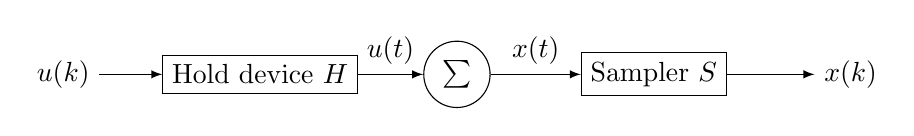
\begin{tikzpicture}[auto, node distance=2.5cm, >=latex]
    % Nodes
    \node (u) {$u(k)$};
    \node [rectangle, draw, right of=u] (H) {Hold device $H$};
    \node [circle, draw, right of=H] (sum) {$\sum$};
    \node [rectangle, draw, right of=sum] (S) {Sampler $S$};
    \node (x) [right of=S] {$x(k)$};

    % Connections with labels
    \draw [->] (u) -- (H);
    \draw [->] (H) -- node[above] {$u(t)$} (sum);
    \draw [->] (sum) -- node[above] {$x(t)$} (S);
    \draw [->] (S) -- (x);
\end{tikzpicture}
\end{center}

\begin{itemize}
    \item \(S\) is the \textbf{sampler} that samples the continuous-time state at intervals \(T\): \(x(k)=x(kT)\).  
    \item \(H\) is the \textbf{hold device} (e.g., zero-order hold) that converts the discrete input \(u(k)\) into a piecewise constant continuous-time signal \(u(t)\).  
    \item The summation block represents the \textbf{continuous-time plant} \(\dot{x}=f(x,u)\).  
    \item The discrete-time summation \(\sum_d\) combines the sampler and hold, giving the discrete evolution:
    \[
    x(k+1) = F(x(k), u(k), T) \approx f_d(x(k),u(k)).
    \]
\end{itemize}

\subsection{Case 1: LTI Plants}\index{Discretization!LTI Plants}

Consider a linear time-invariant (LTI) system:
\[
\dot{x}(t) = A x(t) + B u(t), \quad x(0) = x_0.
\]

Using the zero-order hold over the sampling interval \(T\), the solution is
\[
x((k+1)T) = e^{A T} x(kT) + \int_{0}^{T} e^{A\tau} B u((k+1)T - \tau) \, d\tau.
\]

If \(u(t)\) is piecewise constant \(u(t) = u(k)\) for \(kT \le t < (k+1)T\), the integral simplifies:
\[
\int_0^T e^{A \tau} B u(k) \, d\tau = \left(\int_0^T e^{A \tau} d\tau \right) B u(k),
\]
so the discrete-time model is
\[
\boxed{x(k+1) = e^{A T} x(k) + \left( \int_0^T e^{A \tau} d\tau \right) B u(k)}.
\]

\subsection{Case 2: Nonlinear Plants}\index{Discretization!Nonlinear Plants}

For a nonlinear system
\[
\dot{x} = f(x,u),
\]
a simple forward Euler approximation over the sampling interval \(T\) gives:
\[
\boxed{x(k+1) \approx x(k) + T f(x(k), u(k))}.
\]

This is a first-order discrete-time approximation suitable for small \(T\) and is widely used in digital control of nonlinear systems.

\section{Stability of Discrete-Time Systems}\index{Stability of Discrete-Time Systems}

\subsection{Definitions}\index{Stability of Discrete-Time Systems!Definitions}
\begin{definition}[Stability Concepts]
Consider the discrete-time system $x(k+1) = f(x(k),k)$ with equilibrium $x=0$.  
\begin{itemize}
    \item \textbf{Stable:} For every $\epsilon>0$ there exists $\delta>0$ such that
    \[
    ||x(k_0)|| < \delta \;\; \Rightarrow \;\; ||x(k)|| < \epsilon, \quad \forall k \ge k_0.
    \]
    \item \textbf{Convergent:} $x(k) \to 0$ as $k \to \infty$.
    \item \textbf{Asymptotically Stable:} The equilibrium is stable and convergent.  
    \item \textbf{Unstable:} The equilibrium is not stable.  
\end{itemize}
\end{definition}

\begin{definition}[Uniform Stability Concepts]
The equilibrium $x=0$ is said to be uniformly stable if the $\delta$ in the stability definition is independent of $k_0$.  
\begin{itemize}
    \item \textbf{Uniformly Stable:} $\delta = \delta(\epsilon)$ independent of $k_0$.  
    \item \textbf{Uniformly Convergent:} For every $\epsilon>0$, there exists $N(\epsilon)>0$ independent of $k_0$ such that
    \[
    k \ge k_0 + N(\epsilon) \;\; \Rightarrow \;\; ||x(k)|| < \epsilon.
    \]
    \item \textbf{Uniformly Asymptotically Stable (UAS):} Uniformly stable and uniformly convergent.  
    \item \textbf{Globally Uniformly Asymptotically Stable (GUAS):} Uniformly asymptotically stable with region of attraction $\mathbb{R}^n$.  
\end{itemize}
\end{definition}

\begin{definition}[Exponential Stability]
The equilibrium $x=0$ is \textbf{exponentially stable} if there exist constants $\alpha>0$, $\lambda>0$ such that
\[
||x(k)|| \leq \alpha \, ||x(k_0)|| (1-\lambda)^{k-k_0}, \quad \forall k \ge k_0, \; ||x(k_0)|| < \delta.
\]
If the inequality holds for all $x(k_0)\in\mathbb{R}^n$, the equilibrium is \textbf{globally exponentially stable}.
\end{definition}

%------------------------------------------------
\subsection{Discrete-Time Positive Definite Functions}\index{Stability of Discrete-Time Systems!Discrete-Time Positive Definite Functions}
Let $W : D \times \mathbb{Z}^+ \to \mathbb{R}$ be a scalar function, where $D \subseteq \mathbb{R}^n$ contains the origin. Assume $W(x,k)$ is continuous in $x$ for each $k$.  

\begin{definition}[Positive Semi-Definite Function]
$W(x,k)$ is \textbf{positive semi-definite} in $D$ if
\[
W(0,k) = 0, \quad W(x,k) \ge 0, \;\; \forall x\in D, k \in \mathbb{Z}^+.
\]
\end{definition}

\begin{definition}[Positive Definite Function]
$W(x,k)$ is \textbf{positive definite} if
\[
W(0,k) = 0, \quad W(x,k) > 0 \;\; \forall x \neq 0,
\]
and there exists a continuous function $V_1(x)$ with $V_1(0)=0$ such that
\[
V_1(x) \leq W(x,k), \quad \forall x \in D, k \in \mathbb{Z}^+.
\]
\end{definition}

\begin{definition}[Decrescent Function]
$W(x,k)$ is \textbf{decrescent} in $D$ if there exists a continuous function $V_2(x)$ with $V_2(0)=0$ such that
\[
W(x,k) \leq V_2(x), \quad \forall x \in D, k \in \mathbb{Z}^+.
\]
\end{definition}

\begin{definition}[Radially Unbounded Function]
$W(x,k)$ is \textbf{radially unbounded} if
\[
||x|| \to \infty \;\; \Rightarrow \;\; W(x,k) \to \infty, \quad \forall k \in \mathbb{Z}^+.
\]
\end{definition}

\begin{example}[Discrete-Time Positive Definite Function]
Consider
\[
W(x,k) = (1+0.5\cos k)\|x\|^2, \quad x\in\mathbb{R}^n, k \ge 0.
\]

\begin{itemize}
    \item \textbf{Positive semi-definite:} $W(x,k) \ge 0$.  
    \item \textbf{Positive definite:} $W(0,k) = 0$ and $W(x,k) > 0$ for $x \neq 0$.  
    \item \textbf{Decrescent:} $W(x,k) \le 1.5\|x\|^2$, take $V_2(x)=1.5\|x\|^2$.  
    \item \textbf{Radially unbounded:} As $\|x\|\to \infty$, $W(x,k)\to\infty$.  
\end{itemize}
\end{example}

%------------------------------------------------
\subsection{Stability Theorems}\index{Stability of Discrete-Time Systems!Stability Theorems}

\begin{theorem}[Lyapunov Stability Theorem for Discrete-Time Systems]
If $W:D \times \mathbb{Z}^+ \to \mathbb{R}$ is positive definite and
\[
\Delta W(x(k)) = W(x(k+1),k+1) - W(x(k),k) \le 0,
\]
then the equilibrium $x=0$ is \textbf{stable}.
\end{theorem}

\begin{theorem}[Uniform Asymptotic Stability for Discrete-Time Systems]
If $W(x,k)$ is positive definite, decrescent, and
\[
\Delta W(x(k)) < 0, \quad x\neq 0,
\]
then the equilibrium $x=0$ is \textbf{uniformly asymptotically stable}.
\end{theorem}

\begin{theorem}[Global Uniform Asymptotic Stability]
If $W(x,k)$ is positive definite, decrescent, radially unbounded, and
\[
\Delta W(x(k)) < 0, \quad x\neq 0,
\]
then the equilibrium $x=0$ is \textbf{globally uniformly asymptotically stable}.
\end{theorem}

\begin{remark}\textbf{Hierarchy of Discrete-Time Stability}
\[
\text{GUAS} \;\Rightarrow\; \text{UAS} \;\Rightarrow\; \text{Asymptotic Stability} \;\Rightarrow\; \text{Stability}.
\]
The converse implications do not hold in general.
\end{remark}


\part{FEEDBACK AND STABILITY}

\part{ENERGY-BASED METHODS}

\part{ADVANCED CONTROL DESIGN}

\part{EXAMPLE FILES}
\chapterimage{orange3.jpg} % Chapter heading image
\chapterspaceabove{6.25cm} % Whitespace from the top of the page to the chapter title on chapter pages
\chapterspacebelow{7.5cm} % Amount of vertical whitespace from the top margin to the start of the text on chapter pages

%------------------------------------------------
\chapter{In-text Element Examples}

\section{Referencing Publications}\index{Citation}

This statement requires citation \cite{Smith:2022jd}; this one is more specific \cite[162]{Smith:2021qr}.

%------------------------------------------------

\section{Link Examples}\index{Links}

This is a URL link: \href{https://www.latextemplates.com}{LaTeX Templates}. This is an email link: \href{mailto:example@example.com}{example@example.com}. This is a monospaced URL link: \url{https://www.LaTeXTemplates.com}.

%------------------------------------------------

\section{Lists}\index{Lists}

Lists are useful to present information in a concise and/or ordered way.

\subsection{Numbered List}\index{Lists!Numbered List}

\begin{enumerate}
	\item First numbered item
	\begin{enumerate}
		\item First indented numbered item
		\item Second indented numbered item
		\begin{enumerate}
			\item First second-level indented numbered item
		\end{enumerate}
	\end{enumerate}
	\item Second numbered item
	\item Third numbered item
\end{enumerate}

\subsection{Bullet Point List}\index{Lists!Bullet Points}

\begin{itemize}
	\item First bullet point item
	\begin{itemize}
		\item First indented bullet point item
		\item Second indented bullet point item
		\begin{itemize}
			\item First second-level indented bullet point item
		\end{itemize}
	\end{itemize}
	\item Second bullet point item
	\item Third bullet point item
\end{itemize}

\subsection{Descriptions and Definitions}\index{Lists!Descriptions and Definitions}

\begin{description}
	\item[Name] Description
	\item[Word] Definition
	\item[Comment] Elaboration
\end{description}

%------------------------------------------------

\section{International Support}

àáâäãåèéêëìíîïòóôöõøùúûüÿýñçčšž

\noindent ÀÁÂÄÃÅÈÉÊËÌÍÎÏÒÓÔÖÕØÙÚÛÜŸÝÑ

\noindent ßÇŒÆČŠŽ

%------------------------------------------------

\section{Ligatures}

fi fj fl ffl ffi Ty

\chapterimage{orange2.jpg} % Chapter heading image
\chapterspaceabove{6.25cm} % Whitespace from the top of the page to the chapter title on chapter pages
\chapterspacebelow{7.5cm} % Amount of vertical whitespace from the top margin to the start of the text on chapter pages

%------------------------------------------------
\chapter{Mathematics}

\section{Theorems}\index{Theorems}

\subsection{Several equations}\index{Theorems!Several Equations}

This is a theorem consisting of several equations.

\begin{theorem}[Name of the theorem] % Specify a name/title in square brackets, or leave them out for no title
	In $E=\mathbb{R}^n$ all norms are equivalent. It has the properties:
	\begin{align}
		& \big| ||\mathbf{x}|| - ||\mathbf{y}|| \big|\leq || \mathbf{x}- \mathbf{y}||\\
		&  ||\sum_{i=1}^n\mathbf{x}_i||\leq \sum_{i=1}^n||\mathbf{x}_i||\quad\text{where $n$ is a finite integer}
	\end{align}
\end{theorem}

\subsection{Single Line}\index{Theorems!Single Line}

This is a theorem consisting of just one line.

\begin{theorem} % Specify a name/title in square brackets, or leave them out for no title
	A set $\mathcal{D}(G)$ in dense in $L^2(G)$, $|\cdot|_0$. 
\end{theorem}

%------------------------------------------------

\section{Definitions}\index{Definitions}

A definition can be mathematical or it could define a concept.

\begin{definition}[Definition name] % Specify a name/title in square brackets, or leave them out for no title
	Given a vector space $E$, a norm on $E$ is an application, denoted $||\cdot||$, $E$ in $\mathbb{R}^+=[0,+\infty[$ such that:
	\begin{align}
		& ||\mathbf{x}||=0\ \Rightarrow\ \mathbf{x}=\mathbf{0}\\
		& ||\lambda \mathbf{x}||=|\lambda|\cdot ||\mathbf{x}||\\
		& ||\mathbf{x}+\mathbf{y}||\leq ||\mathbf{x}||+||\mathbf{y}||
	\end{align}
\end{definition}

%------------------------------------------------

\section{Notations}\index{Notations}

\begin{notation} % Specify a name/title in square brackets, or leave them out for no title
	Given an open subset $G$ of $\mathbb{R}^n$, the set of functions $\varphi$ are:
	\begin{enumerate}
		\item Bounded support $G$;
		\item Infinitely differentiable;
	\end{enumerate}
	a vector space is denoted by $\mathcal{D}(G)$. 
\end{notation}

%------------------------------------------------

\section{Remarks}\index{Remarks}

This is an example of a remark.

\begin{remark}
	The concepts presented here are now in conventional employment in mathematics. Vector spaces are taken over the field $\mathbb{K}=\mathbb{R}$, however, established properties are easily extended to $\mathbb{K}=\mathbb{C}$.
\end{remark}

%------------------------------------------------

\section{Corollaries}\index{Corollaries}

\begin{corollary}[Corollary name] % Specify a name/title in square brackets, or leave them out for no title
	The concepts presented here are now in conventional employment in mathematics. Vector spaces are taken over the field $\mathbb{K}=\mathbb{R}$, however, established properties are easily extended to $\mathbb{K}=\mathbb{C}$.
\end{corollary}

%------------------------------------------------

\section{Propositions}\index{Propositions}

\subsection{Several equations}\index{Propositions!Several Equations}

\begin{proposition}[Proposition name] % Specify a name/title in square brackets, or leave them out for no title
	It has the properties:
	\begin{align}
		& \big| ||\mathbf{x}|| - ||\mathbf{y}|| \big|\leq || \mathbf{x}- \mathbf{y}||\\
		&  ||\sum_{i=1}^n\mathbf{x}_i||\leq \sum_{i=1}^n||\mathbf{x}_i||\quad\text{where $n$ is a finite integer}
	\end{align}
\end{proposition}

\subsection{Single Line}\index{Propositions!Single Line}

\begin{proposition} % Specify a name/title in square brackets, or leave them out for no title
	Let $f,g\in L^2(G)$; if $\forall \varphi\in\mathcal{D}(G)$, $(f,\varphi)_0=(g,\varphi)_0$ then $f = g$. 
\end{proposition}

%------------------------------------------------

\section{Examples}\index{Examples}

\subsection{Equation Example}\index{Examples!Equation}

\begin{example} % Specify a name/title in square brackets, or leave them out for no title
	Let $G=\{x\in\mathbb{R}^2:|x|<3\}$ and denoted by: $x^0=(1,1)$; consider the function:
	\begin{equation}
	f(x)=\left\{\begin{aligned} & \mathrm{e}^{|x|} & & \text{si $|x-x^0|\leq 1/2$}\\
	& 0 & & \text{si $|x-x^0|> 1/2$}\end{aligned}\right.
	\end{equation}
	The function $f$ has bounded support, we can take $A=\{x\in\mathbb{R}^2:|x-x^0|\leq 1/2+\epsilon\}$ for all $\epsilon\in\mathopen{]}0\,;5/2-\sqrt{2}\mathclose{[}$.
\end{example}

\subsection{Text Example}\index{Examples!Text}

\begin{example}[Example name] % Specify a name/title in square brackets, or leave them out for no title
	Aliquam arcu turpis, ultrices sed luctus ac, vehicula id metus. Morbi eu feugiat velit, et tempus augue. Proin ac mattis tortor. Donec tincidunt, ante rhoncus luctus semper, arcu lorem lobortis justo, nec convallis ante quam quis lectus. Aenean tincidunt sodales massa, et hendrerit tellus mattis ac. Sed non pretium nibh. Donec cursus maximus luctus. Vivamus lobortis eros et massa porta porttitor.
\end{example}

%------------------------------------------------

\section{Exercises}\index{Exercises}

\begin{exercise} % Specify a name/title in square brackets, or leave them out for no title
	This is a good place to ask a question to test learning progress or further cement ideas into students' minds.
\end{exercise}

%------------------------------------------------

\section{Problems}\index{Problems}

\begin{problem} % Specify a name/title in square brackets, or leave them out for no title
	What is the average airspeed velocity of an unladen swallow?
\end{problem}

%------------------------------------------------

\section{Vocabulary}\index{Vocabulary}

Define a word to improve a students' vocabulary.

\begin{vocabulary}[Word] % Specify a name/title in square brackets, or leave them out for no title
	Definition of word.
\end{vocabulary}
\chapterimage{orange3.jpg} % Chapter heading image
\chapterspaceabove{6.25cm} % Whitespace from the top of the page to the chapter title on chapter pages
\chapterspacebelow{7.5cm} % Amount of vertical whitespace from the top margin to the start of the text on chapter pages

%------------------------------------------------

\chapter{Presenting Information and Results with a Long Chapter Title}

\section{Table}\index{Table}

Lorem ipsum dolor sit amet, consectetur adipiscing elit. Praesent porttitor arcu luctus, imperdiet urna iaculis, mattis eros. Pellentesque iaculis odio vel nisl ullamcorper, nec faucibus ipsum molestie. Sed dictum nisl non aliquet porttitor. Etiam vulputate arcu dignissim, finibus sem et, viverra nisl. Aenean luctus congue massa, ut laoreet metus ornare in. Nunc fermentum nisi imperdiet lectus tincidunt vestibulum at ac elit. Nulla mattis nisl eu malesuada suscipit.

\begin{table}[H] % Use [H] to suppress floating and place the figure/table exactly where it is specified in the text
	\centering % Horizontally center the table on the page
	\begin{tabular}{L{0.15\textwidth} R{0.15\textwidth} R{0.15\textwidth}} % Specify column alignment with L{width}, C{width} and R{width} for fixed-width columns, or the default latex l, c and r for flexible-width columns
		\toprule
		\textbf{Treatments} & \textbf{Response 1} & \textbf{Response 2}\\
		\midrule
		Treatment 1 & 0.0003262 & 0.562 \\
		Treatment 2 & 0.0015681 & 0.910 \\
		Treatment 3 & 0.0009271 & 0.296 \\
		\bottomrule
	\end{tabular}
	\caption{Table caption.}
	\label{tab:example} % Unique label used for referencing the table in-text
\end{table}

Referencing \autoref{tab:example} in-text using its label.

\begin{table}[t] % Floating table, [t] tells LaTeX to place it at the top of the next available page
	\centering % Horizontally center the table on the page
	\begin{tabular}{L{0.15\textwidth} R{0.15\textwidth} R{0.15\textwidth}} % Specify column alignment with L{width}, C{width} and R{width} for fixed-width columns, or the default latex l, c and r for flexible-width columns
		\toprule
		\textbf{Treatments} & \textbf{Response 1} & \textbf{Response 2}\\
		\midrule
		Treatment 1 & 0.0003262 & 0.562 \\
		Treatment 2 & 0.0015681 & 0.910 \\
		Treatment 3 & 0.0009271 & 0.296 \\
		\bottomrule
	\end{tabular}
	\caption{Floating table.}
	\label{tab:floating} % Unique label used for referencing the table in-text
\end{table}

%------------------------------------------------

\section{Figure}\index{Figure}

Lorem ipsum dolor sit amet, consectetur adipiscing elit. Praesent porttitor arcu luctus, imperdiet urna iaculis, mattis eros. Pellentesque iaculis odio vel nisl ullamcorper, nec faucibus ipsum molestie. Sed dictum nisl non aliquet porttitor. Etiam vulputate arcu dignissim, finibus sem et, viverra nisl. Aenean luctus congue massa, ut laoreet metus ornare in. Nunc fermentum nisi imperdiet lectus tincidunt vestibulum at ac elit. Nulla mattis nisl eu malesuada suscipit.

\begin{figure}[H] % Use [H] to suppress floating and place the figure/table exactly where it is specified in the text
	\centering % Horizontally center the figure on the page
	
\includegraphics[width=0.5\textwidth]{creodocs_logo.pdf} % Include the figure image
	\caption{Figure caption.}
	\label{fig:placeholder} % Unique label used for referencing the figure in-text
\end{figure}

Referencing \autoref{fig:placeholder} in-text using its label.

\begin{figure}[b] % Floating figure, [b] tells LaTeX to place it at the bottom of the next available page
	\centering % Horizontally center the figure on the page
	
\includegraphics[width=\textwidth]{creodocs_logo.pdf} % Include the figure image
	\caption{Floating figure.}
	\label{fig:floating} % Unique label used for referencing the figure in-text
\end{figure}


\stopcontents[part] % Manually stop the 'part' table of contents here so the previous Part page table of contents doesn't list the following chapters

%----------------------------------------------------------------------------------------
%	BIBLIOGRAPHY
%----------------------------------------------------------------------------------------

\chapterimage{} % Chapter heading image
\chapterspaceabove{2.5cm} % Whitespace from the top of the page to the chapter title on chapter pages
\chapterspacebelow{2cm} % Amount of vertical whitespace from the top margin to the start of the text on chapter pages

%------------------------------------------------

\chapter*{Bibliography}
\markboth{\sffamily\normalsize\bfseries Bibliography}{\sffamily\normalsize\bfseries Bibliography} % Set the page headers to display a Bibliography chapter name
\addcontentsline{toc}{chapter}{\textcolor{ocre}{Bibliography}} % Add a Bibliography heading to the table of contents

\section*{Articles}
\addcontentsline{toc}{section}{Articles} % Add the Articles subheading to the table of contents

\printbibliography[heading=bibempty, type=article] % Output article bibliography entries

\section*{Books}
\addcontentsline{toc}{section}{Books} % Add the Books subheading to the table of contents

\printbibliography[heading=bibempty, type=book] % Output book bibliography entries

%----------------------------------------------------------------------------------------
%	INDEX
%----------------------------------------------------------------------------------------

\cleardoublepage % Make sure the index starts on an odd (right side) page
\phantomsection
\addcontentsline{toc}{chapter}{\textcolor{ocre}{Index}} % Add an Index heading to the table of contents
\printindex % Output the index

%----------------------------------------------------------------------------------------
%	APPENDICES
%----------------------------------------------------------------------------------------



\begin{appendices}

\renewcommand{\chaptername}{Appendix} % Change the chapter name to Appendix, i.e. "Appendix A: Title", instead of "Chapter A: Title" in the headers

\chapterimage{orange2.jpg} % Chapter heading image
\chapterspaceabove{6.75cm} % Whitespace from the top of the page to the chapter title on chapter pages
\chapterspacebelow{7.25cm} % Amount of vertical whitespace from the top margin to the start of the text on chapter pages
%------------------------------------------------

\chapter{Appendix Sample}

\section{Appendix Section Title}

Lorem ipsum dolor sit amet, consectetur adipiscing elit. Aliquam auctor mi risus, quis tempor libero hendrerit at. Duis hendrerit placerat quam et semper. Nam ultricies metus vehicula arcu viverra, vel ullamcorper justo elementum. Pellentesque vel mi ac lectus cursus posuere et nec ex. Fusce quis mauris egestas lacus commodo venenatis. Ut at arcu lectus. Donec et urna nunc. Morbi eu nisl cursus sapien eleifend tincidunt quis quis est. Donec ut orci ex. Praesent ligula enim, ullamcorper non lorem a, ultrices volutpat dolor. Nullam at imperdiet urna. Pellentesque nec velit eget est euismod pretium.

%------------------------------------------------
\chapterimage{orange2.jpg} % Chapter heading image
\chapterspaceabove{6.75cm} % Whitespace from the top of the page to the chapter title on chapter pages
\chapterspacebelow{7.25cm} % Amount of vertical whitespace from the top margin to the start of the text on chapter pages
%------------------------------------------------
\chapter{Matheemaatics}

\section{Appendix Section Title}

Lorem ipsum dolor sit amet, consectetur adipiscing elit. Aliquam auctor mi risus, quis tempor libero hendrerit at. Duis hendrerit placerat quam et semper. Nam ultricies metus vehicula arcu viverra, vel ullamcorper justo elementum. Pellentesque vel mi ac lectus cursus posuere et nec ex. Fusce quis mauris egestas lacus commodo venenatis. Ut at arcu lectus. Donec et urna nunc. Morbi eu nisl cursus sapien eleifend tincidunt quis quis est. Donec ut orci ex. Praesent ligula enim, ullamcorper non lorem a, ultrices volutpat dolor. Nullam at imperdiet urna. Pellentesque nec velit eget est euismod pretium.

\end{appendices}


\end{document}
